%%
%% Copyright (c) 2017-2018 The Authors.  All Rights Reserved.
%%
%% Weitian LI, et al.
%% School of Physics and Astronomy, Shanghai Jiao Tong University, Shanghai, China.
%%
%% 2017-07-18
%%

\documentclass[modern]{aastex62}
%\documentclass[twocolumn]{aastex62}
%%
%% Defaults: single spaced, 10 point font article
%%
%%  twocolumn   : two text columns, 10 point font, single spaced article.
%%                This is the most compact and represent the final published
%%                derived PDF copy of the accepted manuscript from the publisher
%%  manuscript  : one text column, 12 point font, double spaced article.
%%  preprint    : one text column, 12 point font, single spaced article.
%%  preprint2   : two text columns, 12 point font, single spaced article.
%%  modern      : a stylish, single text column, 12 point font, article with
%%                wider left and right margins. This uses the Daniel
%%                Foreman-Mackey and David Hogg design.
%%
%% Note that you can submit to the AAS Journals in any of these 6 styles.
%%
%% There are other optional arguments one can envoke to allow other stylistic
%% actions. The available options are:
%%
%%  astrosymb    : Loads Astrosymb font and define \astrocommands.
%%  tighten      : Makes baselineskip slightly smaller, only works with
%%                 the twocolumn substyle.
%%  times        : uses times font instead of the default
%%  linenumbers  : turn on lineno package.
%%  trackchanges : required to see the revision mark up and print its output
%%  longauthor   : Do not use the more compressed footnote style (default) for
%%                 the author/collaboration/affiliations. Instead print all
%%                 affiliation information after each name. Creates a much
%%                 long author list but may be desirable for short author papers

%% Extra packages
\usepackage{amsmath}
\usepackage{csquotes}  % `enquote'
\usepackage{bm}  % bold math
\usepackage{savesym}

\savesymbol{tablenum}  % workaround symbol conflict
                       % credit: https://tex.stackexchange.com/a/269074
\usepackage{siunitx}  % typeset units; from `texlive-science'
\restoresymbol{SI}{tablenum}  % `tablenum' from `siunitx' becomes `SItablenum'

%% Graphics
% Credit: https://tex.stackexchange.com/a/45502
\usepackage{grfext}
\PrependGraphicsExtensions*{.png,.PNG}  % prefer PNG figures
\graphicspath{{./}{figures/}}  % NOTE: the trailing '/' matters

%% Chinese
\usepackage{xeCJK}
\setCJKmainfont{Noto Serif CJK SC}[BoldFont=Noto Sans CJK SC]
\setCJKsansfont{Noto Sans CJK SC}
\setCJKmonofont{Noto Sans Mono CJK SC}

%% Bibliography style
\bibliographystyle{aasjournal-links}

%% Custom macros
\newcommand{\R}[1]{\mathrm{#1}}
\newcommand{\D}[1]{\R{d} #1}
\newcommand{\diff}[2]{\frac{\D{#1}}{\D{#2}}}
\newcommand{\pdiff}[2]{\frac{\partial #1}{\partial #2}}
\newcommand{\lcdm}{$\Lambda$CDM}
\newcommand{\Halpha}{\text{H$\alpha$}}
\newcommand{\Hi}{H\textsc{i}}
\newcommand{\Hii}{H\textsc{ii}}
\newcommand{\klos}{\text{$k_{\parallel}$}}
\newcommand{\kperp}{\text{$k_{\bot}$}}
\newcommand{\fov}{\text{Fo\!V}}
% Credit: https://tex.stackexchange.com/a/2230
\makeatletter
\newcommand{\rms}{r.m.s\@ifnextchar.{}{.\@}}
\makeatother

%% Marks
\newcommand{\NOTE}[1]{\textcolor{violet}{[\textbf{NOTE:}~\uwave{#1}]}}
\newcommand{\TODO}[1]{\textcolor{magenta}{[\textbf{TODO:}~\uuline{#1}]}}
\newcommand{\OK}[1]{\textcolor{cyan}{[\textbf{OK:}~\uline{#1}]}}
\newcommand{\XU}[1]{\textcolor{blue}{[\textbf{XU:}~\uline{#1}]}}
\newcommand{\LI}[1]{\textcolor{purple}{[\textbf{LI:}~\uline{#1}]}}

%% Custom math operators (requires `amsmath' package)
\DeclareMathOperator{\erf}{erf}
\DeclareMathOperator{\erfc}{erfc}

%% Settings for package `siunitx'
% credit: https://tex.stackexchange.com/a/194042
\sisetup{
  range-phrase=\text{--},
  range-units=single,
  product-units=power,
  list-separator={, },
  list-final-separator={, and },
}
%
%% Custom units (requires `siunitx' package)
\DeclareSIUnit\arcsec{arcsec}
\DeclareSIUnit\arcmin{arcmin}
\DeclareSIUnit\cMpc{cMpc}  % comoving Mpc
\DeclareSIUnit\cGpc{cGpc}  % comoving Gpc
\DeclareSIUnit\deg{deg}
\DeclareSIUnit\erg{erg}
\DeclareSIUnit\gauss{G}
\DeclareSIUnit\hour{hr}  % overwrite hour from 'h' to 'hr'
\DeclareSIUnit\hubble{\text{$h$}}
\DeclareSIUnit\jansky{Jy}
\DeclareSIUnit\lightyear{ly}
\DeclareSIUnit\parsec{pc}
\DeclareSIUnit\rayleigh{Rayleigh}
\DeclareSIUnit\solarmass{\text{M$_{\odot}$}}
\DeclareSIUnit\year{yr}
%
\DeclareSIUnit\keV{\kilo\electronvolt}
\DeclareSIUnit\kpc{\kilo\parsec}
\DeclareSIUnit\mJy{\milli\jansky}
\DeclareSIUnit\mK{\milli\kelvin}
\DeclareSIUnit\uG{\micro\gauss}
\DeclareSIUnit\Gyr{\giga\year}
\DeclareSIUnit\MHz{\mega\hertz}
\DeclareSIUnit\Mpc{\mega\parsec}
\DeclareSIUnit\Gpc{\giga\parsec}

%% Hyperref-related settings
\def\sectionautorefname{Section}
\def\subsectionautorefname{Section}
\def\subsubsectionautorefname{Section}
\def\figureautorefname{Figure}
\def\tableautorefname{Table}
% Credit: https://tex.stackexchange.com/a/66150
\def\equationautorefname~#1\null{Equation~(#1)\null}

%% Custom subsubsubsection ...
\newcounter{sssseccount}
\newcommand{\sssseclabel}{\alph{sssseccount}}
\newcommand{\ssssec}[1]{%
  \vspace{1ex}%
  \stepcounter{sssseccount}%
  \noindent\emph{\sssseclabel. #1}%
}

%% Custom settings
\setlength{\parindent}{1.5em}

%% Journal information
\received{2018 ???}
\revised{???}
\accepted{???}
\submitjournal{ApJ}

%% Add a light gray and diagonal water-mark to the first page
%\watermark{DRAFT}  % watermark text: DRAFT
%% Control the water-mark size with:
%% \setwatermarkfontsize{dimension}

%% Short title to be used as the running head (<= 44 characters)
%%          ............................................
\shorttitle{Contamination of Radio Halos on EoR Signal}
\shortauthors{Li~\textit{et~al.}}


%%%%%%%%%%%%%%%%%%%%%%%%%%%%%%%%%%%%%%%%%%%%%%%%%%%%%%%%%%%%%%%%%%%%%%%%%

\begin{document}

\title{\bfseries%
  \color{cyan}%
  Evaluating the Contamination of Radio Halos
  on the Epoch of Reionization Observations
}

%% The \author command is the same as before except it now takes an optional
%% argument which is the 16 digit ORCID.  The syntax is:
%% \author[xxxx-xxxx-xxxx-xxxx]{Author Name}
%%
%% This will hyperlink the author name to the author's ORCID page. Note that
%% during compilation, LaTeX will do some limited checking of the format of
%% the ID to make sure it is valid.
%%
%% Use \affiliation for affiliation information.  Please use multiple
%% \affiliation calls for to document more than one affiliation.  AASTeX v6.1
%% will automatically index these in the header.  When a duplicate is found
%% its index will be the same as its previous entry.
%%
%% The new \altaffiliation can be used to indicate some secondary information
%% such as fellowships. This command produces a non-numeric footnote that is
%% set away from the numeric \affiliation footnotes.  NOTE that if an
%% \altaffiliation command is used it must come BEFORE the \affiliation call,
%% right after the \author command, in order to place the footnotes in
%% the proper location.
%%
%% Use \email to set provide email addresses. Each \email will appear on its
%% own line so you can put multiple email address in one \email call.
%%
%% A new \correspondingauthor command is available in V6.1 to identify the
%% corresponding author of the manuscript.  It is the author's responsibility
%% to make sure this name is also in the author list.
%%
%% While authors can be grouped inside the same \author and \affiliation
%% commands it is better to have a single author for each.  This allows for
%% one to exploit all the new benefits and should make book-keeping easier.
%%
%% If done correctly the peer review system will be able to automatically
%% put the author and affiliation information from the manuscript and save
%% the corresponding author the trouble of entering it by hand.

\correspondingauthor{Haiguang Xu}
\email{hgxu@sjtu.edu.cn}

\author[0000-0002-7527-380X]{Weitian Li}
\email{liweitianux@sjtu.edu.cn}
\affiliation{School of Physics and Astronomy,
  Shanghai Jiao Tong University,
  800 Dongchuan Road, Shanghai 200240, China}

\author{Haiguang Xu}
\affiliation{School of Physics and Astronomy,
  Shanghai Jiao Tong University,
  800 Dongchuan Road, Shanghai 200240, China}
\affiliation{Tsung-Dao Lee Institute,
  Shanghai Jiao Tong University,
  800 Dongchuan Road, Shanghai 200240, China}
\affiliation{IFSA Collaborative Innovation Center,
  Shanghai Jiao Tong University,
  800 Dongchuan Road, Shanghai 200240, China}

\author[0000-0003-1263-9453]{Zhixian Ma}
\affiliation{Department of Electronic Engineering,
  Shanghai Jiao Tong University,
  800 Dongchuan Road, Shanghai 200240, China}
\author{Dan Hu}
\affiliation{School of Physics and Astronomy,
  Shanghai Jiao Tong University,
  800 Dongchuan Road, Shanghai 200240, China}
\author{Zhenghao Zhu}
\affiliation{School of Physics and Astronomy,
  Shanghai Jiao Tong University,
  800 Dongchuan Road, Shanghai 200240, China}
\author{Chenxi Shan}
\affiliation{School of Physics and Astronomy,
  Shanghai Jiao Tong University,
  800 Dongchuan Road, Shanghai 200240, China}
\author{Jingying Wang}
\affiliation{Department of Physics and Astronomy,
  University of the Western Cape,
  Cape Town 7535, South Africa}
\author[0000-0001-9765-6521]{Junhua Gu}
\affiliation{National Astronomical Observatories,
  Chinese Academy of Sciences,
  20A Datun Road, Beijing 100012, China}
\author{Xiaoli Lian}
\affiliation{School of Physics and Astronomy,
  Shanghai Jiao Tong University,
  800 Dongchuan Road, Shanghai 200240, China}
\author{Qian Zheng}
\affiliation{Shanghai Astronomical Observatory,
  Chinese Academy of Sciences,
  80 Nandan Road, Shanghai 200030, China}
\author{Jie Zhu}
\affiliation{Department of Electronic Engineering,
  Shanghai Jiao Tong University,
  800 Dongchuan Road, Shanghai 200240, China}

%%%%%%%%%%%%%%%%%%%%%%%%%%%%%%%%%%%%%%%%%%%%%%%%%%%%%%%%%%%%%%%%%%%%%%%%%

%% The abstract should summarize concisely the content and conclusions
%% of the article.  The abstract should be a single paragraph of not more
%% than 250 words.

\begin{abstract}
\noindent
The overwhelming foreground contamination is one of the primary
impediments to probing the Epoch of Reionization (EoR) through measuring
the redshifted 21~cm signal.
Among the various foreground components, radio halos in galaxy clusters
are less studied and their impacts on the EoR observations are still
poorly known.
In this work, we employ the merger-induced turbulence re-acceleration
model to simulate the low-frequency emissions of radio halos, and
generate the \enquote{observed} images by adopting the latest SKA1-Low
layout configuration to incorporate the practical instrumental effects.
{\color{cyan}%
The calculated one-dimensional power spectra show that radio
halos can be generally about \numlist{e4;e3;e2} times stronger than the
EoR signal in the \numrange{120}{128}, \numrange{154}{162}, and
\numrange{192}{200} \si{\MHz} bands, respectively.
By calculating the two-dimensional power spectra and defining the EoR
windows, the power ratios of radio halos to the EoR signal can
still be up to about \SIrange[range-units=repeat]{1000}{2000}{\percent},
\SIrange[range-units=repeat]{30}{100}{\percent}, and
\SIrange[range-units=repeat]{10}{80}{\percent} in the three bands
within the typical \SI{68}{\percent} error bars that are caused by
the number density uncertainties of bright radio halos.
Moreover, radio halos inside the far side-lobes of the station beam
can impose strong contamination inside the EoR window.
In conclusion, we argue that radio halos are severe foreground sources
to the EoR detection and require serious treatment in the forthcoming
deep EoR observations.
}
% ~??? words
\end{abstract}

%% Authors should select subject keywords from the given list.  No more
%% than 6 keywords should be given, and they should be listed in
%% alphabetical order.
%%
%% See the online documentation for the full list of available subject
%% keywords and the rules for their use.
%% http://journals.aas.org/authors/keywords2013.html
\keywords{%
  dark ages, reionization, first stars ---
  early universe ---
  galaxies: clusters: intracluster medium ---
  methods: data analysis ---
  techniques: interferometric
}


%########################################################################
\section{Introduction}
\label{sec:intro}
%########################################################################

The Epoch of Reionization (EoR; $z \sim \numrange{6}{15}$) refers to
a period of our Universe preceded by the Cosmic Dawn
($z \sim \numrange{15}{30}$) and the Dark Ages ($z \sim \numrange{30}{200}$)
and is expected to last from about 300 million to about 1 billion years
after the Big Bang \citep[see][and references therein]{koopmans2015rev}.
During the EoR, the reionization of
neutral hydrogen (\Hi) that is caused primarily by the ultra-violet and
soft X-ray photons emitted from the first generation celestial objects
efficiently surpassed the cooling of the gas through
recombination of electrons and protons.
As a result, the majority of baryonic matter was again in a
highly ionized state.
Comparing with the observations of distant quasars and cosmic microwave
background (CMB), which have provided some important but loose
constraints on the reionization process \citep[see][for a review]{fan2006rev},
the 21~cm line emission from \Hi{} is recognized to be the decisive probe
to directly explore the EoR
\citep[see][for reviews]{furlanetto2006rev,zaroubi2013rev,furlanetto2016rev}.

In order to probe the EoR, a number of radio interferometers working
at the low-frequency radio bands (\SIrange{\sim 50}{200}{\MHz}) have been
designed to target the redshifted 21~cm signal, among which there are
the Square Kilometre Array (SKA; \citealt{mellema2013rev,koopmans2015rev}),
the Hydrogen Epoch of Reionization Array (HERA; \citealt{deboer2017}),
and their pathfinders, such as
the LOw Frequency ARray (LOFAR; \citealt{vanHaarlem2013}),
the Murchison Widefield Array (MWA; \citealt{bowman2013,tingay2013}),
the Precision Array for Probing the Epoch of Reionization
(PAPER; \citealt{parsons2010}),
and the 21 CentiMeter Array (21CMA; \citealt{zheng2016}).
The challenges met in these experiments, however, are immense
due to a variety of complicated instrumental effects,
ionospheric distortions, radio frequency interference, and the
strong celestial foreground contamination, which overwhelms the
redshifted 21~cm signal by about \numrange{4}{5} orders of magnitude
\citep[see][for a review]{morales2010rev}.

Among various contaminating foreground components, the Galactic diffuse
radiation (including both the synchrotron and free-free emissions)
and extragalactic point sources are the most prominent and contribute
the majority of the foreground contamination
\citep[e.g.,][]{shaver1999,diMatteo2004,gleser2008,liu2012,murray2017,spinelli2018}.
At about \SI{150}{\MHz}, it is estimated that they may account for
about \SI{71}{\percent} and \SI{27}{\percent} of the total foreground
contamination, respectively \citep{shaver1999}.
Most of the remaining foreground arises from the synchrotron emission
from the extragalactic diffuse sources that include the large-scale
filaments embedded in the cosmic webs,
the intergalactic medium located at the cluster outskirts,
and the intracluster medium (ICM) of galaxy clusters (radio halos,
radio relics, and mini-halos).
Although these sources are less constrained by observations, especially
in the low-frequency regime, it is estimated that they are tens to
hundreds of times brighter than the EoR signal and hence impede
the EoR detection \citep[e.g.,][]{waxman2000,diMatteo2004,gleser2008}.
For example, \citet{diMatteo2004} calculated that the intensity
fluctuation caused by radio halos and relics is about three orders of
magnitude larger than that of the EoR signal at \SI{115}{\MHz}.
Consequently, a careful treatment of the extragalactic diffuse sources
is indispensable in order to extract the elusive EoR signal.

In this work, we attempt to address this issue by focusing on the
evolution of diffuse radio halos in galaxy clusters via detailed
modeling and their impacts on detecting the EoR signal.
First discovered in the Coma cluster \citep{large1959}, radio halos
have been observed in about 80 merging galaxy clusters roughly at
their centers, showing relatively regular morphologies and spatial
extensions of $\sim\,$\si{\Mpc}, as well as an obvious correlation
with the X-ray-emitting ICM \citep[e.g.,][]{cassano2013}.
It should be noted that the angular sizes of radio halos happen to be
several to tens of arcminutes, which coincide with those theoretically
predicted for the ionizing bubbles during the EoR.
This, complemented with the potentially large number (several to tens
of thousands in the whole sky) of radio halos to be revealed by the
forthcoming low-frequency radio telescopes \citep[e.g.,][]{cassano2015},
indicates that to better guide foreground removal and avoidance methods,
it is essential to investigate the cumulative emission of radio halos as
a foreground contaminating source \citep[e.g.,][]{diMatteo2004,gleser2008}.
As of today, however, only very few works have been dedicated to this
topic and are all based on relatively straightforward modeling methods,
e.g., using the \SI{1.4}{\GHz} radio flux function or radio--X-ray
scaling relations, which are barely constrained by current observations
\citep[e.g.,][]{gleser2008,jelic2008}.
The data acquired in these observations are far from complete due to
the lack of systematic surveys targeting these diffuse sources,
especially in the low-frequency radio bands \citep[e.g.,][]{kale2016rev}.

This paper is prepared as follows.
In \autoref{sec:sky-simu} we simulate the low-frequency radio sky, among
which a detailed simulation of radio halos in galaxy clusters has been
developed by applying the merger-induced turbulence re-acceleration model.
In \autoref{sec:obs-simu} we employ the latest SKA1-Low layout
configuration to incorporate the practical instrumental effects into
the simulated sky maps.
We briefly introduce the power spectra and the EoR window in
\autoref{sec:ps-eorw}
and then quantitatively evaluate the contamination caused by radio halos
on the EoR measurements in \autoref{sec:results}.
In \autoref{sec:discussions}, we discuss how the EoR measurements are
affected by the instrumental frequency artifacts and by the radio halos
inside the far side-lobes of the station beam.
Finally, we summarize our work in \autoref{sec:summary}.
Throughout this work we adopt a flat \lcdm{} cosmology with
$H_0 = \SI{100}{\hubble} = \SI{71}{\km\per\second\per\Mpc}$,
$\Omega_m = 0.27$, $\Omega_{\Lambda} = 1 - \Omega_m = 0.73$,
$\Omega_b = 0.046$, $n_s = 0.96$, and $\sigma_8 = 0.81$.
The quoted errors are at \SI{68}{\percent} confidence level unless
otherwise stated.


%########################################################################
\section{Simulation of Low-Frequency Radio Sky}
\label{sec:sky-simu}
%########################################################################

Based on our previous works \citep{wang2010,wang2013}, we have developed
the \texttt{FG21sim}\footnote{%
  FG21sim: \url{https://github.com/liweitianux/fg21sim}}
software to simulate the low-frequency
radio sky by taking into account the contributions of our Galaxy,
extragalactic point sources, and radio halos in galaxy clusters.
We choose three representative frequency bands, namely
\numrange{120}{128}, \numrange{154}{162}, and \numrange{192}{200}
\si{\MHz}, and perform simulations for a sky patch of size
\SI[product-units=repeat]{10 x 10}{\degree}.
The \SI{8}{\MHz} bandwidth is chosen to limit the effect of
cosmological evolution of the EoR signal when calculating power
spectra \citep[e.g.][]{wyithe2004,thyagarajan2013}.
The simulated sky maps are pixelized into \num{1800 x 1800} with a pixel
size of \SI{20}{\arcsecond}.
The simulation parameters are also listed in \autoref{tab:freq-bands}.

\begin{deluxetable}{cccc}
\tablecaption{\label{tab:freq-bands}%
  Simulation Parameters for the Three Bands
}
\tablehead{
  \colhead{Frequency band (\si{\MHz})} &
  \colhead{\numrange{120}{128}} &
  \colhead{\numrange{154}{162}} &
  \colhead{\numrange{192}{200}}
}
\startdata
Central frequency ($f_c$) & \SI{124}{\MHz} & \SI{158}{\MHz} & \SI{196}{\MHz} \\
EoR redshift range &
  \numrange{10.10}{10.84} & \numrange{7.77}{8.22} & \numrange{6.10}{6.40} \\
Bandwidth ($B$) & \multicolumn{3}{c}{\SI{8}{\MHz}} \\
Region size &
  \multicolumn{3}{c}{\SI[product-units=repeat]{10 x 10}{\degree}} \\
Image size & \multicolumn{3}{c}{\num{1800x1800}} \\
Pixel size & \multicolumn{3}{c}{\SI{20}{\arcsecond}}
\enddata
\end{deluxetable}


%========================================================================
\subsection{Radio Halos in Galaxy Clusters}
\label{sec:cluster-halos}
%========================================================================

As a significant improvement over our past works \citep{wang2010,wang2013},
we consider in detail the evolution of radio halos in galaxy clusters
by employing the merger-induced turbulence re-acceleration model,
in terms of which the relativistic electrons in the ICM are re-accelerated
by the turbulence generated in merger events via the second-order Fermi
process, and lose energies due to mechanisms including synchrotron
radiation, inverse Compton scattering off the CMB photons, and Coulomb
collisions with the thermal ICM \citep[see][for a review]{brunetti2014rev}.
For a galaxy cluster, we first employ the extended Press-Schechter
theory to simulate its merging history, and then calculate the turbulent
acceleration efficiency and duration for each merger event.
By combining the effects of turbulent acceleration and energy loss,
we obtain the temporal evolution of the relativistic electron spectrum,
from which we calculate the synchrotron radiation of the radio halo.

%------------------------------------------------------------------------
\subsubsection{Mass Function}
\label{sec:mass-function}
%------------------------------------------------------------------------

The Press-Schechter formalism was originally advanced as one of the standard
method to predict the mass function of galaxy clusters and its evolution
in the Universe \citep{press1974}, and has been extended to combine with
the cold dark matter (CDM) models \citep[e.g.,][]{bond1991,lacey1993}.
In this formalism, the number of galaxy clusters per unit comoving volume
at redshift $z$ with masses in the range from $M$ to $M + \R{d}M$ is
\begin{equation}
  \label{eq:ps-mass-func}
  n(M, z) \,\D{M} = \sqrt{\frac{2}{\pi}} \frac{\langle{\rho}\rangle}{M}
  \frac{\delta_c(z)}{\sigma^2(M)} \left| \diff{\sigma(M)}{M} \right|
  \exp\!\left[ -\frac{\delta_c^2(z)}{2\sigma^2(M)} \right] \D{M},
\end{equation}
where $M$ is the virial mass of galaxy clusters,
$\langle {\rho} \rangle$ is the current mean density of the Universe,
$\delta_c(z)$ is the critical linear overdensity for a region to collapse
at redshift $z$ [see \autoref{eq:delta-crit}],
and $\sigma(M)$ is the current root-mean-square (\rms) density
fluctuations within a sphere of mean mass $M$.

Considering the CDM model and the mass range covered by galaxy clusters,
it is reasonable to adopt the following power-law distribution for the
density perturbations \citep{sarazin2002,randall2002}
\begin{equation}
  \label{eq:sigma-mass}
  \sigma(M) = \sigma_8 \left( \frac{M}{M_8} \right)^{-\alpha},
\end{equation}
where $\sigma_8$ is the current \rms{} density fluctuations on
a scale of \SI{8}{\per\hubble\Mpc},
$M_8 = (4\pi/3)(8 \,\si{\per\hubble\Mpc})^3 \langle{\rho}\rangle$
is the mass contained in a sphere of a radius \SI{8}{\per\hubble\Mpc},
and the exponent $\alpha = (n+3)/6$ with $n = -7/5$ \citep{randall2002}
is related to the fluctuation pattern whose power spectrum varies
with wavenumber $k$ as $k^n$.

Using a minimum galaxy cluster mass of
$M_{\R{min}} = \SI{e14}{\solarmass}$
and a maximum redshift cut at $z_{\R{max}} = 4$,
we apply \autoref{eq:ps-mass-func} to derive the total number of
galaxy clusters in a given sky patch, together with the mass and
redshift distributions.
The galaxy cluster sample is then built by randomly drawing mass and
redshift pairs $(M_{\R{sim}}, z_{\R{sim}})$ from these distributions.

%------------------------------------------------------------------------
\subsubsection{Merging History}
\label{sec:merging-history}
%------------------------------------------------------------------------

Galaxy clusters are formed hierarchically through accretion and mergers.
The extended Press-Schechter theory outlined in \citet{lacey1993} provides
a way to describe their growth history in terms of the merger tree.
In order to build the merger tree for a galaxy cluster, we start with
its \enquote{current} mass $M_{\R{sim}}$ and redshift $z_{\R{sim}}$ obtained
in \autoref{sec:mass-function}, and trace its growth history back in time
by running Monte Carlo simulations to randomly determine the mass change
$\Delta M$ at each step, which may be regarded either as a merger event
(if $\Delta M > \Delta M_c$) or as an accretion event
(if $\Delta M \leq \Delta M_c$).
Considering that radio halos are usually associated with major mergers,
we choose $\Delta M_c = \SI{e13}{\solarmass}$ \citep[e.g.,][]{cassano2005}.

We assume that during each growth step the cluster mass increases
from $M_1$ at time $t_1$ to $M_2$ at a later time $t_2$ ($> t_1$).
Given $M_2$ and $t_2$, the conditional probability of the cluster had
a progenitor being in the mass range $[M_1, M_1 + \D{M_1}]$ at an
earlier time $t_1$ can be expressed as
\begin{equation}
  \label{eq:eps-condprob}
  \R{Pr}(M_1, t_1 | M_2, t_2) \,\D{M_1} = \frac{1}{\sqrt{2\pi}}
  \frac{M_2}{M_1}
  \frac{\delta_{c1} - \delta_{c2}}{(\sigma_1^2 - \sigma_2^2)^{3/2}}
  \left| \diff{\sigma_1^2}{M_1} \right|
  \exp \!\left[ -\frac{(\delta_{c1} - \delta_{c2})^2}
    {2(\sigma_1^2 - \sigma_2^2)} \right] \D{M_1},
\end{equation}
where
$\delta_{ci} \equiv \delta_c(t_i)$, $\sigma_i \equiv \sigma(M_i)$, and $i =
1, 2$ is used to denote parameters defined at time $t_1$ and $t_2$,
respectively \citep{lacey1993,randall2002}.
By further introducing $S \equiv \sigma^2(M)$ and
$\omega \equiv \delta_c(t)$, this equation reduces to
\begin{equation}
  \label{eq:eps-condprob-simp}
  \R{Pr}(\Delta S, \Delta \omega) \,\D{\Delta S} = \frac{1}{\sqrt{2\pi}}
  \frac{\Delta\omega}{(\Delta S)^{3/2}}
  \exp \!\left[ -\frac{(\Delta\omega)^2}{2 \Delta S} \right] \D{\Delta S}.
\end{equation}

In order to resolve mergers with a mass change $\Delta M_c \ll M$
during the backward tracing of a galaxy cluster, a time step $\Delta t$
(i.e., $\Delta\omega$) that satisfies
\begin{equation}
  \label{sec:dw-step}
  \Delta\omega \lesssim \Delta\omega_{\R{max}} = \left[
    S \left| \diff{\ln \sigma^2}{\ln M} \right|
    \left( \frac{\Delta M_c}{M} \right) \right]^{1/2}
\end{equation}
is required \citep{lacey1993}, and we adopt an adaptive step of
$\Delta\omega = \Delta\omega_{\R{max}} / 2$ \citep{randall2002}.
At a certain step when $\Delta\omega$ is given, the mass change
$\Delta S$ can be randomly drawn from the following cumulative
probability distribution of sub-cluster masses
\begin{equation}
  \label{sec:cdf-sub-masses}
  \R{Pr}(<\!\Delta S, \Delta\omega) =
  \int_0^{\Delta S} \R{Pr}(\Delta S', \Delta\omega) \,\D{\Delta S'} =
  \erfc \!\left( \frac{\Delta \omega}{\sqrt{2 \Delta S}} \right),
\end{equation}
where $\erfc(x) = 1 - \erf(x)$ is the complementary error function,
and the cluster's progenitor mass $M_1$ is then obtained as
$S_1 = S_2 + \Delta S$.

Given that observable radio halos are regarded to be associated
with recent (in the frame of the observer) major mergers
and have typical lifetimes $\tau_{\R{halo}} \lesssim \SI{1}{\Gyr}$
at \SI{1.4}{\GHz} \citep[e.g.,][]{brunetti2009,cassano2016},
we trace the merging history of each galaxy cluster by a maximum
backward time of \SI{3}{\Gyr} from its \enquote{current} age
$t_{\R{sim}}$ (corresponding to $z_{\R{sim}}$).
For each built merger tree, we extract the information of all
the mergers associated with the main cluster to carry out the
following radio halo simulation.


%------------------------------------------------------------------------
\subsubsection{Radio Halo Emergence and Evolution}
\label{sec:halos}
%------------------------------------------------------------------------

According to the re-acceleration model, there exists a population of
primary (or fossil) high-energy electrons, which permeate the ICM and
are thought to be injected by active galactic nucleus (AGN) activities
and star formation \citep[see][for a review]{blasi2007rev}.
When a cluster experiences a merger, the turbulence is generated
throughout the ICM and can accelerate the primary electrons to be highly
relativistic, resulting in the observed radio halo.

In addition to the energy increase that is caused by the turbulent
acceleration, electrons in the ICM lose energy via synchrotron radiation,
inverse Compton scattering off the CMB photons,
Coulomb collisions, etc.\ \citep{sarazin1999}.
For a population of electrons with isotropic energy distribution, the
temporal evolution of the number density distribution $n(\gamma, t)$
is governed by the following Fokker-Planck diffusion-advection equation
\citep{eilek1991,schlickeiser2002}
\begin{equation}
  \label{eq:fokkerplanck}
  \pdiff{n(\gamma,t)}{t} = \pdiff{}{\gamma} \left[ n(\gamma,t) \left(
      \left| \diff{\gamma}{t} \right| -
      \frac{2}{\gamma} D_{\gamma\gamma}(\gamma, t) \right) \right] +
    \pdiff{}{\gamma} \left[ D_{\gamma\gamma} \pdiff{n(\gamma,t)}{\gamma}
    \right] + Q_e(\gamma,t),
\end{equation}
where $\gamma$ is the Lorentz factor of electrons,
$D_{\gamma\gamma}(\gamma, t)$ is the diffusion coefficient describing
the interactions between the turbulence and electrons,
$|\R{d}\gamma / \R{d}t|$ is the energy loss rate,
and $Q_e(\gamma, t)$ describes the electron injection.

%........................................................................
\setcounter{sssseccount}{0}
\ssssec{Thermal Electrons}

The number density of thermal electrons $n_{\R{th}}$ in the ICM can be
calculated as
\begin{equation}
  \label{eq:number-density-thermal}
  n_{\R{th}} \simeq \frac{3 f_b M_{\R{vir}}}{4\pi \mu m_u \,r^3_{\R{vir}}},
\end{equation}
where
$f_b \simeq \Omega_b/\Omega_m$ is the mean baryon fraction assumed for
galaxy clusters,
$M_{\R{vir}}$ is the cluster's virial mass,
$r_{\R{vir}}$ is the virial radius [see \autoref{eq:radius-virial}],
$\mu \simeq 0.6$ is the mean molecular weight \citep[e.g.,][]{ettori2013},
and $m_u$ is the atomic mass unit.
Therefore, the corresponding thermal energy density $\epsilon_{\R{th}}$
of the ICM is given by
\begin{equation}
  \label{eq:energy-density-thermal}
  \epsilon_{\R{th}} = \frac{3}{2} \,n_{\R{th}} \,k_BT_{\R{cl}},
\end{equation}
where the cluster's mean temperature is approximated as the virial
temperature, i.e.,
$k_BT_{\R{cl}} \simeq k_BT_{\R{vir}} = G M_{\R{vir}} \mu m_u / (2 \,r_{\R{vir}})$.

%........................................................................
\ssssec{Electron Injection}

As primary electrons are continuously injected into the ICM by AGN
activities and star formation, it is reasonable to assume an average
injection rate \citep[e.g.,][]{cassano2005,donnert2014} and a power-law
spectrum for the electron injection process
\begin{equation}
  \label{eq:electron-inj}
  Q_e(\gamma, t) \simeq Q_e(\gamma) = K_e \,\gamma^{-s},
\end{equation}
where $s = 2.3$ is the adopted spectral index \citep[e.g.,][]{sarazin1999}.
Moreover, the total energy of the injected electrons is assumed to account
for a fraction ($\eta_e$) of the ICM's total thermal energy
\citep{cassano2005}, i.e.,
\begin{equation}
  \epsilon_e \,\tau_{\R{cl}} \int_{\gamma_{\R{min}}}^{\gamma_{\R{max}}}
  Q_e(\gamma') \gamma' \,\D{\gamma'}
  = \eta_e \,\epsilon_{\R{th}},
\end{equation}
where $\tau_{\R{cl}} \simeq t_{\R{sim}}$ is the cluster's age at its
\enquote{current} redshift $z_{\R{sim}}$ as simulated in
\autoref{sec:mass-function},
and $\epsilon_e = m_e c^2$ is the electron's rest energy.
Given $\gamma_{\R{min}} \ll \gamma_{\R{\max}}$, the injection rate $K_e$
is derived to be
\begin{equation}
  \label{eq:injrate}
  K_e \simeq \frac{(s-2)\,\eta_e\,\epsilon_{\R{th}}}{\epsilon_e\,\tau_{\R{cl}}}
    \gamma_{\R{min}}^{s-2}.
\end{equation}

%........................................................................
\ssssec{Initial Electron Spectrum}

To determine the initial electron spectrum $n_e(\gamma, t_0)$, which will
be used to solve \autoref{eq:fokkerplanck},
we evolve the accumulated electron spectrum
$n_e'(\gamma) = Q_e(\gamma) \,\tau_0$ for \SI{1}{\Gyr} by applying
the same Fokker-Planck equation with the turbulent acceleration turned
off \citep[e.g.,][]{brunetti2007}, where $\tau_0$ is the cluster's age
in the beginning of the first merger and can be approximated as the
starting time of the first merger.

%........................................................................
\ssssec{Turbulent Acceleration}

The details of interactions between the turbulence and both thermal and
relativistic particles are complicated and still poorly understood.
Among several particle acceleration mechanisms that can be potentially
triggered by the turbulence, the most important one is the transit time
damping process, i.e., the turbulence dissipates its energy and
accelerates particles by interacting with the relativistic particles
(e.g., cosmic rays) in the ICM
\citep[and references therein]{brunetti2007,brunetti2011}.
The associated diffusion coefficient is given as
\citep{pinzke2017,miniati2015}
\begin{equation}
  \label{eq:dpp}
  D_{\gamma\gamma} = \gamma^2 \frac{4\pi \zeta}{X_{\R{cr}} L_{\R{turb}}}
    \frac{\langle (\delta{v_t})^2 \rangle^2}{c_s^3},
\end{equation}
where
$\zeta \sim \numrange{0.1}{0.3}$ is an efficiency factor characterizing
the plasma instabilities (e.g., due to spatial or temporal intermittency),
$X_{\R{cr}} = \epsilon_{\R{cr}} / \epsilon_{\R{th}} \sim \SI{1}{\percent}$
is the relative energy density of cosmic rays with respect to the thermal ICM,
$L_{\R{turb}} \simeq r_{\R{vir}}/3$ is the turbulence injection scale
\citep{miniati2015},
$\langle (\delta{v_t})^2 \rangle$ is the turbulence velocity dispersion,
and $c_s = \sqrt{\gamma_{\R{gas}} k_BT_{\R{cl}} / (\mu m_u)}$ is the sound
speed in the ICM with $\gamma_{\R{gas}} = 5/3$ being the adiabatic index
of ideal monatomic gas.

In order to estimate the velocity dispersion of the turbulence, we assume
that a fraction ($\eta_{\R{turb}}$) of the kinetic energy carried by the
merger is transferred into turbulent waves, i.e.,
\begin{equation}
  \label{eq:energy-turb}
  E_{\R{turb}} = \frac{1}{2} M_{\R{turb}}^b
    \langle (\delta{v_t})^2 \rangle = \eta_{\R{turb}} E_{\R{merger}},
\end{equation}
where
$M_{\R{turb}}^b$ is the baryon mass enclosed in the turbulent region
(i.e., within radius of $L_{\R{turb}}$),
and $E_{\R{merger}}$ is merger's kinetic energy, which can be approximated
as the potential energy released from the infalling sub-cluster
\begin{equation}
  \label{eq:energy-merger}
  E_{\R{merger}} \simeq \frac{1}{2} f_b M_{\R{vir,s}} \,v^2_{\R{vir}}
    \simeq \frac{1}{2} f_b M_{\R{vir,s}}
    \frac{G M_{\R{vir,m}}}{r^2_{\R{vir,m}}},
\end{equation}
where
$M_{\R{vir,m}}$ and $r_{\R{vir,m}}$ are the virial mass and radius of the
main cluster, respectively, and $M_{\R{vir,s}}$ is the virial mass of the
sub-cluster.
By adopting the NFW density profile \citep{navarro1997}, the distribution
of mass within a radius of $s \,r_{\R{vir}}$ ($s$ is the normalized radius
in units of the virial radius) in fraction of the virial mass is
\begin{equation}
  \label{eq:mass-dist-nfw}
  f_{\R{nfw}}(s) = \frac{M(< s \,r_{\R{vir}})}{M_{\R{vir}}} =
    \frac{\ln(1 + c s) - c s / (1 + c s)}{\ln(1 + c) - c / (1 + c)},
\end{equation}
where
$c \sim 5$ is the concentration parameter for clusters \citep{lokas2001}.
Therefore we have
\begin{equation}
  \label{eq:mass-turb}
  M_{\R{turb}}^b = f_b M_{\R{merged}}(<L_{\R{turb}})
    = f_b f_{\R{nfw}}(1/3) (M_{\R{vir,m}} + M_{\R{vir,s}}).
\end{equation}
By substituting Equations~(\ref{eq:energy-merger}) and (\ref{eq:mass-turb})
into \autoref{eq:energy-turb}, we obtain the turbulence velocity dispersion
as
\begin{equation}
  \label{eq:turb-velocity-dispersion}
  \langle (\delta{v_t})^2 \rangle =
    \frac{\eta_{\R{turb}}}{f_{\R{nfw}}(1/3)}
    \frac{M_{\R{vir,s}}}{M_{\R{vir,m}} + M_{\R{vir,s}}}
    \frac{G M_{\R{vir,m}}}{r^2_{\R{vir,m}}}.
\end{equation}

Generally, the turbulence generated during major mergers is subsonic
with a Mach number of
$\mathcal{M}_{\R{turb}} = \sqrt{\langle (\delta{v_t})^2 \rangle} / c_s
  \sim \numrange{0.2}{0.5}$.
The acceleration efficiency can be described by the systematic
acceleration timescale (i.e., the reciprocal of the acceleration rate;
e.g., \citealt{brunetti2011})
$\tau_{\R{acc}} = \gamma^2 / (4 D_{\gamma\gamma}) \sim \SI{0.1}{\Gyr}$,
suggesting that the turbulent acceleration may be a moderately efficient
mechanism to accelerate the relativistic electrons in the ICM and be used
to explain the generation of radio halos.

%........................................................................
\ssssec{Acceleration Periods}

The whole merger process may last for \SIrange{2}{3}{\Gyr}
\citep[e.g.,][]{tormen2004,cassano2016},
however, the period $\tau_{\R{turb}}$ that the turbulence is intense and
thus can effectively accelerate particles is relatively short:
$\tau_{\R{turb}} \simeq 2 L_{\R{turb}} / v_{\R{imp}}$,
where $v_{\R{imp}}$ is the relative impact velocity between the merging
clusters \citep{miniati2015}.
Starting from a sufficiently large distance with zero velocity,
the relative impact velocity of two merging clusters with mass
$M_{\R{vir,m}}$ and $M_{\R{vir,s}}$ is given by
\citep{sarazin2002,cassano2005}
\begin{equation}
  \label{eq:v-imp}
  v_{\R{imp}} \simeq \left[
    \frac{2G (M_{\R{vir,m}} + M_{\R{vir,s}})}{r_{\R{vir,m}}}
    \left( 1 - \frac{1}{\eta_v} \right)\right]^{1/2},
\end{equation}
with $\eta_v \simeq 4 \,(1 + M_{\R{vir,s}}/M_{\R{vir,m}})^{1/3}$.
Based on these, we estimate that major mergers generally have an effective
turbulent acceleration duration of $\tau_{\R{turb}} \sim \SI{0.5}{\Gyr}$.

For each merger event
$(M^{(i)}_{\R{vir,m}}, M^{(i)}_{\R{vir,s}}, t^{(i)}_{\R{merger}})$
as simulated in \autoref{sec:merging-history} for a galaxy cluster,
where $t^{(i)}_{\R{merger}}$ denotes the starting time of the $i$-th
merger event, we calculate the corresponding turbulent acceleration
duration $\tau^{(i)}_{\R{turb}}$, and solve the Fokker-Planck equation
by taking into account both turbulent acceleration and energy losses
during the period
$[\,t^{(i)}_{\R{merger}}, t^{(i)}_{\R{merger}}+\tau^{(i)}_{\R{turb}}\,]$.

%........................................................................
\ssssec{Energy Losses}

There are several mechanisms through which the relativistic electrons in
the ICM can lose energies \citep{sarazin1999}, and we take into account
the following three major mechanisms in this work.
The first one is the inverse Compton scattering off the CMB photons,
the energy loss rate of which is
\begin{equation}
  \label{eq:eloss-ic}
  \left( \diff{\gamma}{t} \right)_{\R{IC}} =
    \num{-4.32e-4} \,\gamma^2 (1+z)^4
    \quad [\si{\per\Gyr}].
\end{equation}

Secondly, with the \si{\uG}-level magnetic field permeating the ICM,
relativistic electrons will produce synchrotron radiation and lose
energy at a rate of
\begin{equation}
  \label{eq:eloss-syn}
  \left( \diff{\gamma}{t} \right)_{\R{syn}} =
    \num{-4.10e-5} \,\gamma^2 \left( \frac{B}{\SI{1}{\uG}} \right)^2
    \quad [\si{\per\Gyr}],
\end{equation}
where $B$ is the averaged magnetic field strength.
We assume that the magnetic field is uniform and its energy density
is a fraction of the thermal energy density, i.e.,
$u_B = B^2 / (8\pi) = \eta_B \,\epsilon_{\R{th}}$,
where $\eta_B$ is the energy density ratio between the magnetic field
and the thermal ICM \citep[e.g.,][]{bohringer2016}.

The last mechanism considered here is that relativistic electrons lose
energy by interacting with the thermal electrons via Coulomb collisions,
the energy loss rate of which is
\begin{equation}
  \label{eq:eloss-coul}
  \left( \diff{\gamma}{t} \right)_{\R{Coul}} =
    \num{-3.79e4} \left( \frac{n_{\R{th}}}{\SI{1}{\per\cm\cubed}} \right)
    \left[ 1 + \frac{1}{75} \ln \left(
        \gamma \,\frac{n_{\R{th}}}{\SI{1}{\per\cm\cubed}} \right) \right]
    \quad [\si{\per\Gyr}].
\end{equation}

The inverse Compton scattering and synchrotron radiation dominate
the energy losses at the high-energy regime ($\gamma \gtrsim 1000$),
while Coulomb collisions are the main energy-loss mechanism for electrons
with lower energies ($\gamma \lesssim 100$).
Therefore, electrons with intermediate energies (e.g., $\gamma \sim 300$)
have a very long lifetime (\SI{\sim 3}{\Gyr}) and can accumulate in the
ICM as the cluster grows \citep{sarazin1999}, which may become the primary
electrons to be accelerated \textit{in situ} by the turbulence.

%........................................................................
\ssssec{Numerical Method}

With all the coefficients in \autoref{eq:fokkerplanck} being determined,
we can evolve the initial electron spectrum $n_e(\gamma,\, t_0)$ via
solving the Fokker-Planck equation, and derive the \enquote{current}
electron spectrum $n_e(\gamma,\, t_{\R{sim}})$,
where $t_{\R{sim}}$ corresponds to the simulated redshift $z_{\R{sim}}$
(\autoref{sec:mass-function}).
An efficient numerical method proposed by \citet{chang1970} is utilized
to solve the equation under the no-flux boundary condition \citep{park1996}.
To avoid unphysical pile-up of electrons around the lower boundary caused
by the boundary condition,
we define a \enquote{buffer} region below $\gamma_{\R{buf}}$, within which
the spectral data are replaced by extrapolating the data above
$\gamma_{\R{buf}}$ as a power-law spectrum \citep{donnert2014}.
We adopt a logarithmic grid for $\gamma \in [1, 10^5]$ with 200 cells,
and let the buffer region span 10 cells.

%........................................................................
\ssssec{Image Generation}

After deriving the \enquote{current} electron spectrum
$n_e(\gamma, t_{\R{sim}})$, the synchrotron emissivity at frequency
$\nu$ is given by \citep{rybicki1979}
\begin{equation}
  \label{sec:jnu-sync}
  % unit: [erg/s/Hz/cm^3]
  J_{\R{syn}}(\nu) = \frac{\sqrt{3} \, e^3 B}{m_e c^2}
    \!\int_{\gamma_{\R{min}}}^{\gamma_{\R{max}}} \!\!\!\int_0^{\pi/2}\!
    n_e(\gamma, t_{\R{sim}}) F(\nu/\nu_c)
    \sin^2 \!\theta \,\D{\theta} \,\D{\gamma},
\end{equation}
where $\theta$ is the pitch angle of electrons,
and $F(\nu/\nu_c) = (\nu/\nu_c) \int_{\nu/\nu_c}^{\infty} K_{5/3}(x) \,\D{x}$
is the synchrotron kernel,
with $K_{5/3}(x)$ the modified Bessel function of 5/3 order,
$\nu_c = (3/2) \,\gamma^2 \nu_L \sin\theta
= 3 e B \gamma^2 \sin\theta / (4\pi m_e c)$
the electron's critical frequency.
The simulated radio halo is assumed to be the same size as the turbulent
region \citep[e.g.,][]{vazza2011}:
$r_{\R{halo}} \simeq L_{\R{turb}} \simeq r_{\R{vir}}/3$,
therefore its radio power at a certain frequency (i.e., spectral power) is
\begin{equation}
  \label{eq:halo-power}
  P(\nu) = \frac{4\pi}{3} r_{\R{halo}}^3 J_{\R{syn}}(\nu),
\end{equation}
and its flux density measured at the same frequency is
\begin{equation}
  \label{eq:halo-flux}
  S(\nu) = \frac{(1+z_{\R{sim}}) P(\nu(1+z_{\R{sim}}))}{4\pi D_{\!L}^2(z_{\R{sim}})},
\end{equation}
where $D_{\!L}(z_{\R{sim}})$ is the luminosity distance to the halo at
redshift $z_{\R{sim}}$,
and the factor $(1 + z_{\R{sim}})$ accounts for the $K$ correction
\citep[e.g.,][]{hogg1999}.

To generate the image for the simulated radio halos, we adopt an
exponential profile for the azimuthally averaged brightness distribution
\citep{murgia2009}:
\begin{equation}
  \label{eq:halo-profile}
  I_{\nu}(\theta) = I_{\nu,0} \exp(-3 \,\theta / \theta_{\R{halo}}),
\end{equation}
where $\theta = r / D_{\!A}(z_{\R{sim}})$ is the angular radius from the
halo center with $D_{\!A}(z_{\R{sim}})$ being the angular diameter
distance to the halo,
and $I_{\nu,0} = 9 S(\nu) / (2\pi \theta^2_{\R{halo}})$ is the central
brightness.

%........................................................................
\ssssec{Parameters Tuning}

Our model has the following 5 parameters:
(1) fraction of the merger energy transferred into the turbulence:
$\eta_{\R{turb}} \sim \SI{10}{\percent}$;
(2) relative energy density of the magnetic field:
$\eta_B \sim \SI{0.1}{\percent}$;
(3) ratio of the total energy of injected electrons to the total thermal
energy: $\eta_e \sim \SI{0.1}{\percent}$;
(4) efficiency of the ICM plasma instabilities:
$\zeta \sim 0.1$;
(5) relative energy density in the cosmic rays:
$X_{\R{cr}} \sim \SI{1.5}{\percent}$.
Although all of them have reasonable constraints from either
observational evidences or simulation studies, it is essential to further
tune them in order to achieve better agreement with the observations.
To this end, we have collected all currently observed radio halos
(\autoref{tab:halos-observed}; 71 identified halos and 9 candidates;
as of 2018 January), and compare the
\SI{1.4}{\GHz} all-sky integrated flux function between our simulated
radio halos and the observations.
We have explored various parameter configurations,
and for each configuration we have repeated the simulation for 500 times
in order to take into account the distribution variations of bright
radio halos across the sky.
Considering that the current observations are far from complete,
especially in the low-flux end, our strategy is requiring that the
integrated flux function of simulated radio halos agrees with the
observed one in the high-flux end within error bars.
Consequently, we have chosen a set of model parameters with
$\eta_{\R{turb}} = \SI{10}{\percent}$, $\eta_B = \SI{0.1}{\percent}$,
$\eta_e = \SI{0.3}{\percent}$, $\zeta = 0.1$,
and $X_{\R{cr}} = \SI{1.5}{\percent}$.
A comparison between the \SI{1.4}{\GHz} all-sky integrated flux
functions of radio halos obtained in observations and simulations is
shown in \autoref{fig:halos-simucomp},
where we also plot the \SI{158}{\MHz} all-sky integrated flux function
for the simulated radio halos, which shows that radio halos are much
brighter at lower frequencies.

\begin{figure}
  \centering
  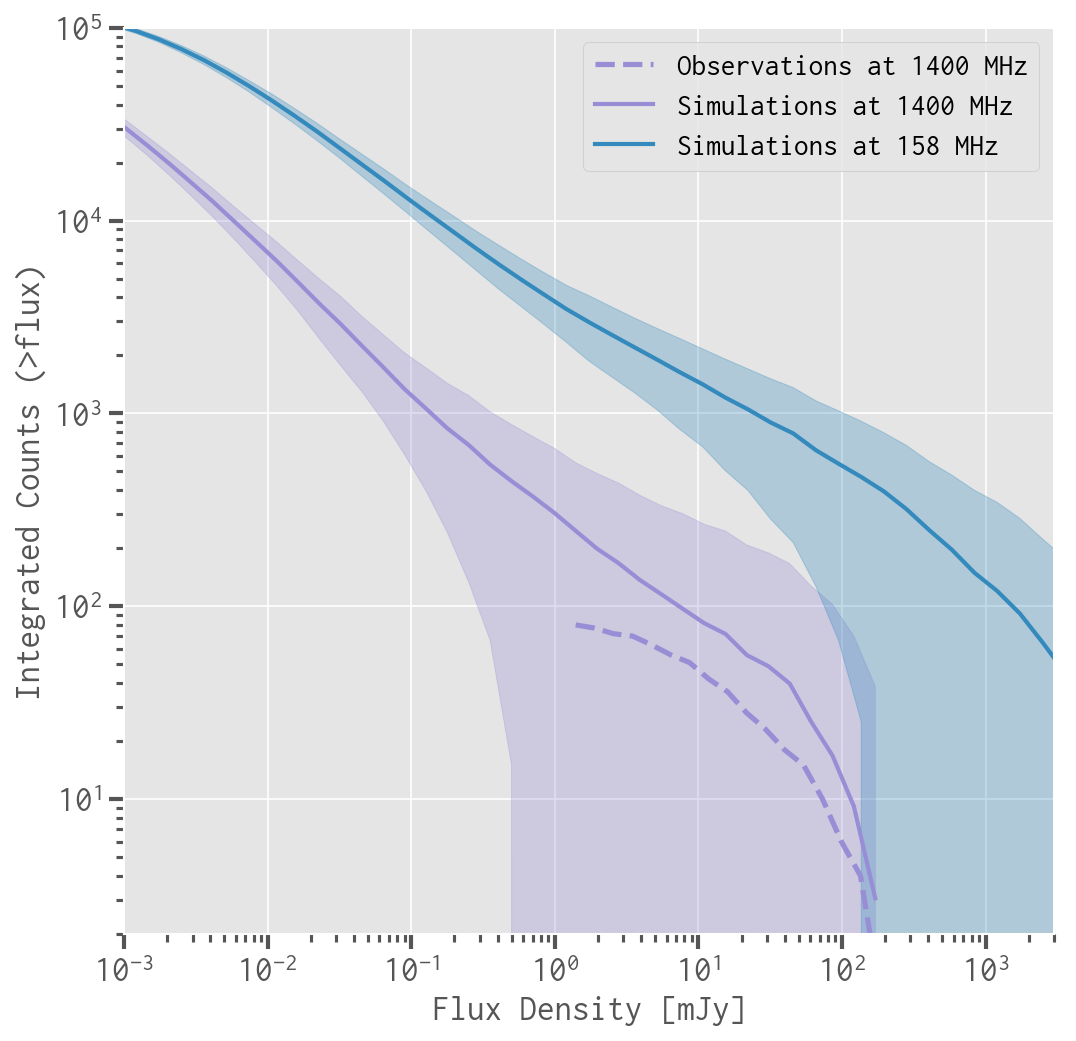
\includegraphics[width=0.6\textwidth]{fluxfunc-simucomp-1400}
  \caption{\label{fig:halos-simucomp}%
    The \SI{1.4}{\GHz} all-sky integrated flux function comparison
    between the observed (purple dashed line) and simulated
    (purple solid line) radio halos.
    The \SI{158}{\MHz} all-sky integrated flux function for the simulated
    halos is also plotted in blue solid line.
    The shaded regions show the \SI{68}{\percent} uncertainties of the
    simulated radio halos derived from the 500 simulation runs.
  }
\end{figure}

In order to describe the uncertainty of the number density of bright
radio halos across the sky, which are generally correlated with massive
galaxy clusters, we repeat the simulation of radio halos for 100 times.
The medians and the corresponding \SI{68}{\percent} uncertainties%
\footnote{The \SI{68}{\percent} uncertainty is derived from the 16th
and 84th percentiles because they are more robust than the mean and
standard deviation for data with large dispersion.}
of the \rms{} brightness temperature are
$\left(6.95_{-5.04}^{+21.0}\right) \times 10^3$ \si{\mK},
$\left(2.75_{-1.97}^{+10.4}\right) \times 10^3$ \si{\mK}, and
$\left(1.24_{-0.92}^{+4.86}\right) \times 10^3$ \si{\mK}
at \numlist{124;158;196} \si{\MHz}, respectively
(\autoref{tab:tb-rms}; see also \autoref{fig:halos-example} for an
example of the simulated radio halos at \SI{158}{\MHz}).

\begin{figure}
  \centering
  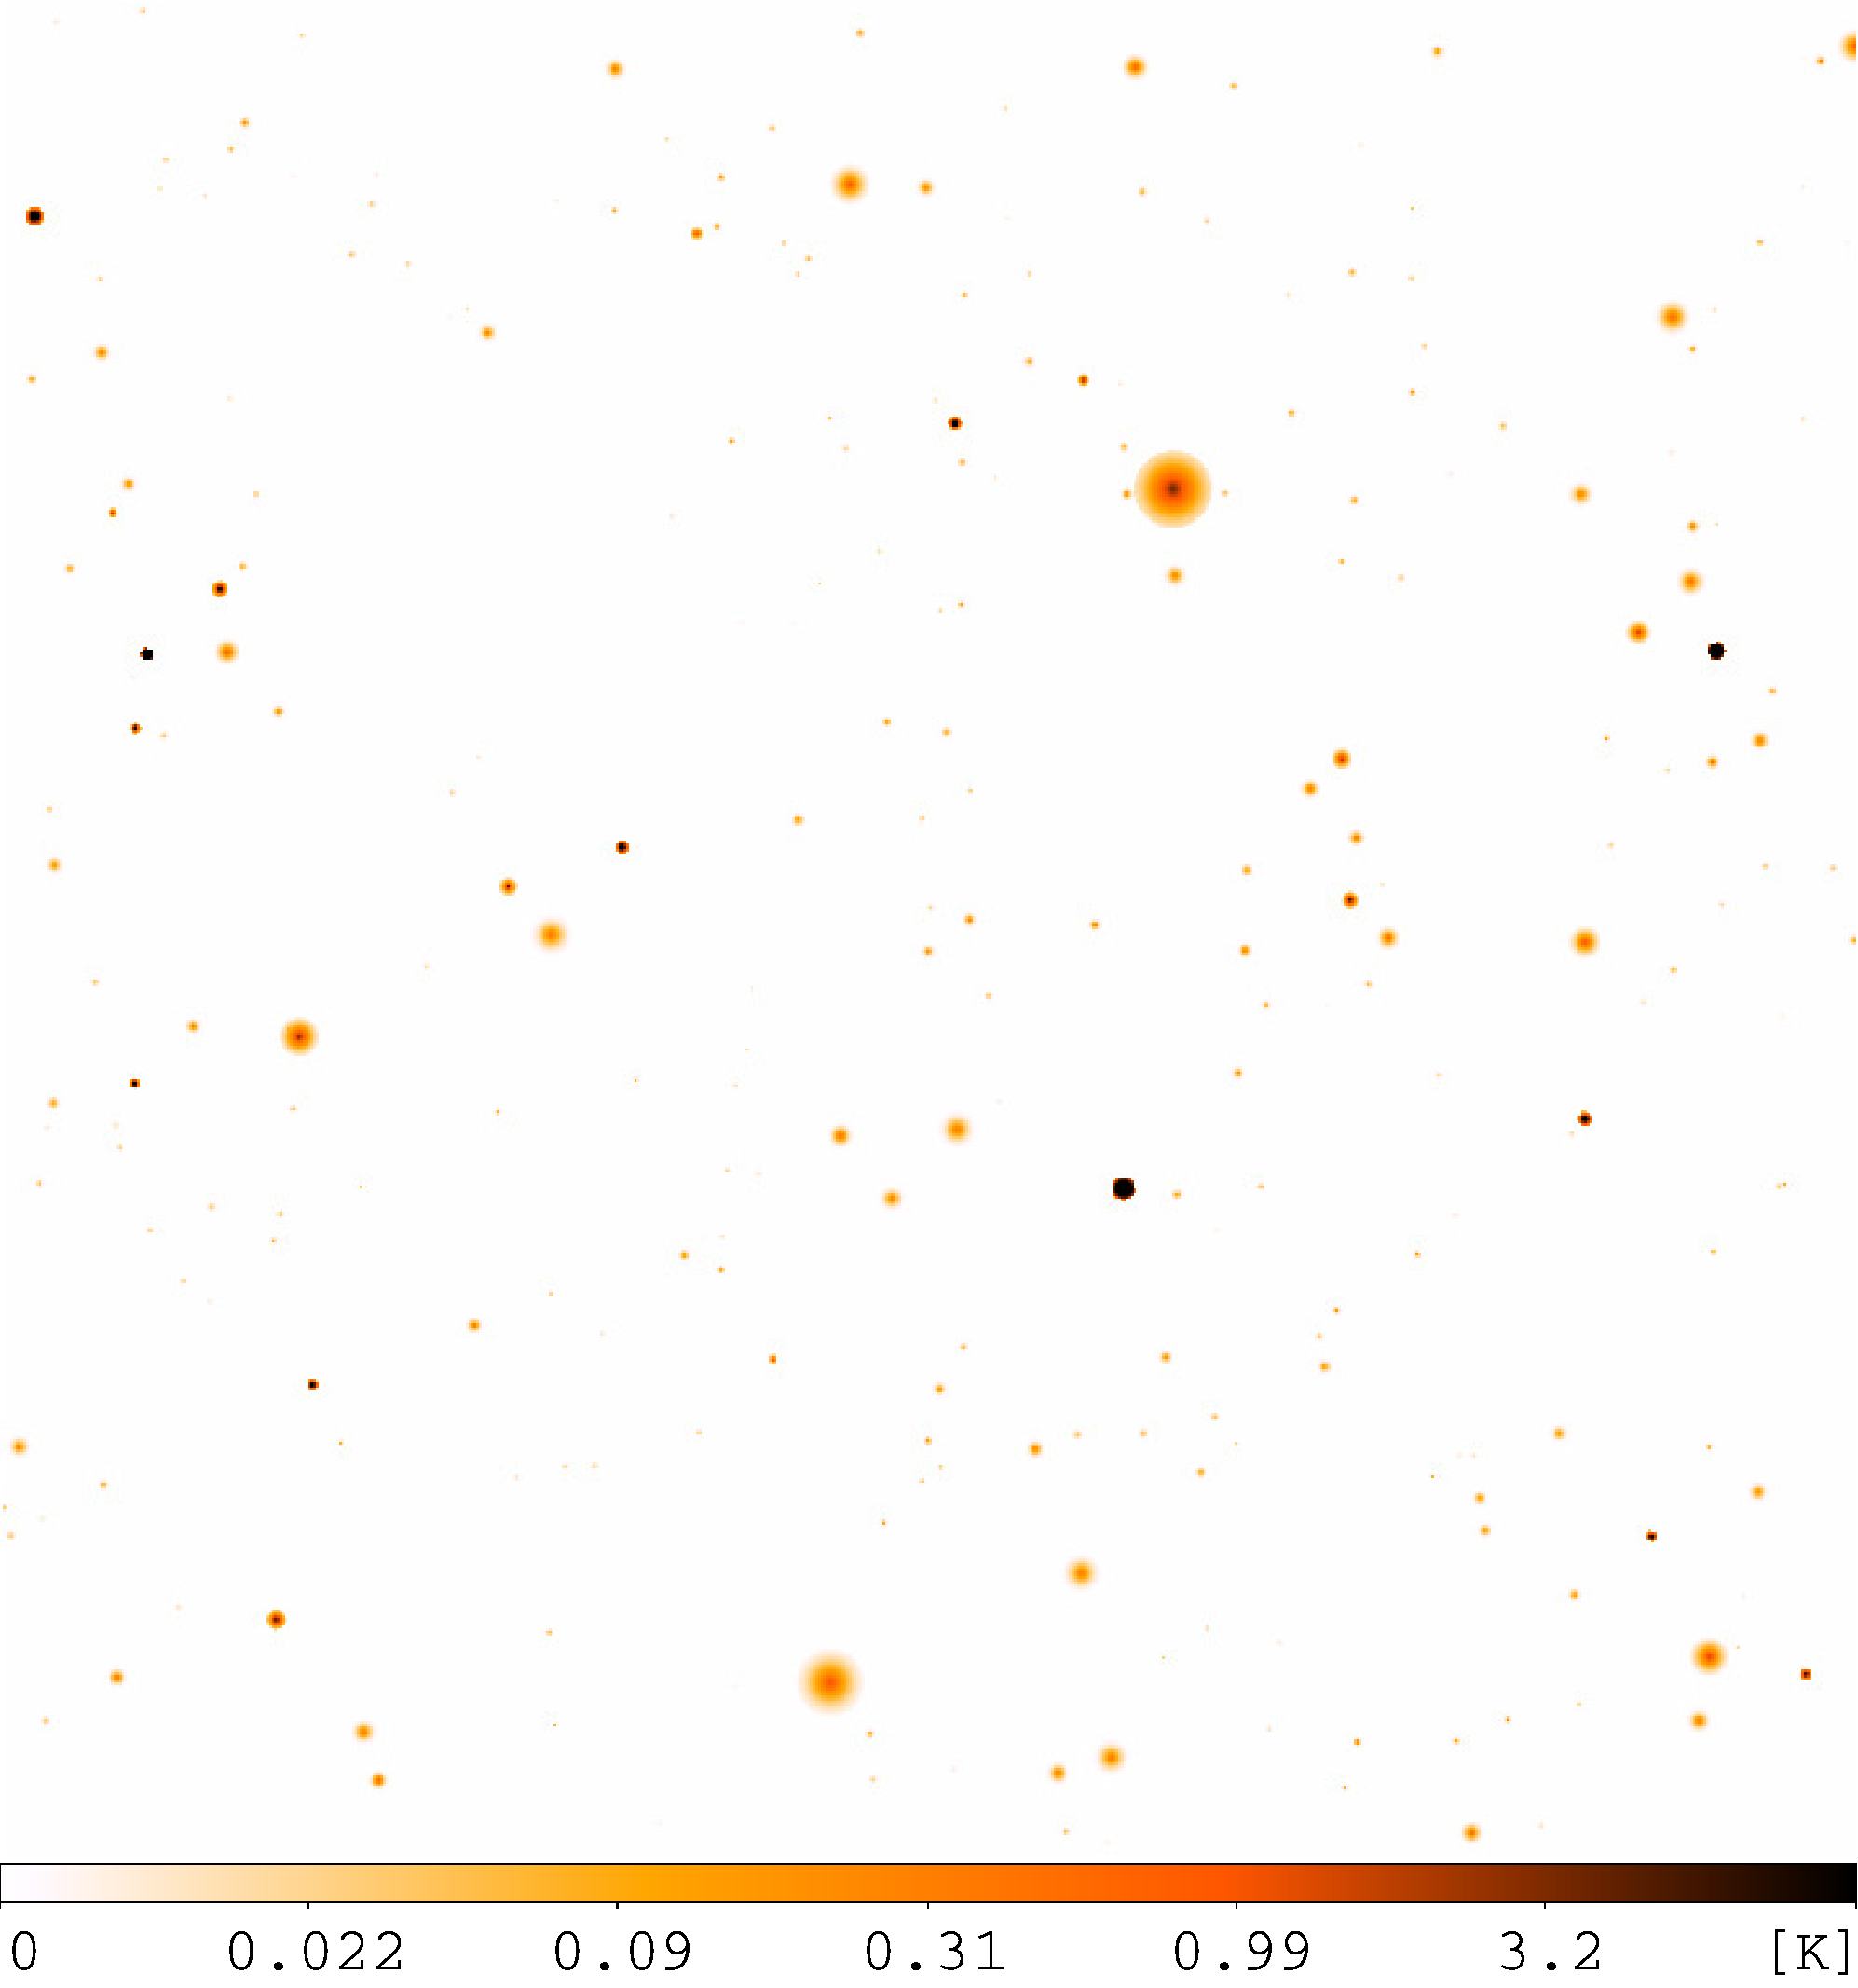
\includegraphics[width=0.6\textwidth]{halos-f158-heat-log2}
  \caption{\label{fig:halos-example}%
    An example from the 100 simulation runs showing the simulated
    radio halos at \SI{158}{\MHz}.
    The sky region size is \SI[product-units=repeat]{10 x 10}{\degree},
    and the color bar is in units of \si{\kelvin}.
  }
\end{figure}

\begin{deluxetable}{cccc}
\tablecaption{\label{tab:tb-rms}%
  The \rms{} Brightness Temperatures of the Foreground Components and
  the EoR Signal (Unit: \si{\mK})
}
\tablehead{
  \colhead{Component} &
  \colhead{\SI{124}{\MHz}} &
  \colhead{\SI{158}{\MHz}} &
  \colhead{\SI{196}{\MHz}}
}
\startdata
Radio halos (100 simulations) &
  $\left(6.95_{-5.04}^{+21.0}\right) \times 10^3$ &
  $\left(2.75_{-1.97}^{+10.4}\right) \times 10^3$ &
  $\left(1.24_{-0.92}^{+4.86}\right) \times 10^3$ \\
Galactic synchrotron & \num{4.74e5} & \num{2.52e5} & \num{1.43e5} \\
Galactic free-free & \num{330} & \num{200} & \num{130} \\
Extragalactic point sources & \num{2.97e8} & \num{5.90e7} & \num{1.39e7} \\
EoR signal & \num{15.1} & \num{11.3} & \num{3.77}
\enddata
\end{deluxetable}


%========================================================================
\subsection{Other Foreground Components}
\label{sec:fg-other}
%========================================================================

Following our previous work \citep{wang2010}, we have also simulated
several other foreground components, including the Galactic synchrotron
and free-free emissions as well as the extragalactic point sources,
in order to carry out comparisons of power spectra between radio halos
and other foreground components as an effort to better characterize the
contributions of radio halos to the low-frequency radio sky.

The Galactic synchrotron map is simulated by extrapolating the
Haslam \SI{408}{\MHz} all-sky map as the template to lower frequencies
with a power-law spectrum.
We make use of the $N_{\R{side}} = 2048$
(pixel size \SI{\sim 1.72}{\arcminute})
high-resolution version of the Haslam \SI{408}{\MHz} map\footnote{%
  The reprocessed Haslam \SI{408}{\MHz} map:
  \url{http://www.jb.man.ac.uk/research/cosmos/haslam_map/}.},
which was reprocessed by \citet{remazeilles2015} using significantly
better instrument calibration and more accurate subtraction of
extragalactic sources.
We also use the all-sky synchrotron spectral index map made by
\citet{giardino2002} to account for the index variation with sky positions.
The Galactic free-free emission is deduced from the \Halpha{} survey
data \citep{finkbeiner2003}, which is corrected for dust absorption,
by employing the tight relation between the \Halpha{} and free-free
emissions due to their common origins
\citep[see][and references therein]{dickinson2003}.
{\color{cyan}%
Since the Galactic diffuse emissions vary remarkably across the sky,
we simulate the Galactic synchrotron and free-free maps at position of
(R.A., Dec.)\ = (\SI{0}{\degree}, \SI{-27}{\degree}), which locates at a
high galactic latitude ($b = \SI{-78.5}{\degree}$) and is expected to be
an appropriate choice for this study (see also \autoref{sec:obs-simu}).}

The extragalactic point sources are simulated by taking into account the
following 5 types of sources: (1) star-forming and starburst galaxies,
(2) radio-quiet AGNs, (3) Fanaroff-Riley type I and type II AGNs,
(4) GHz-peaked spectrum AGNs, and (5) compact steep spectrum AGNs.
We simulate the former three types of sources by leveraging the simulation
results made by \citet{wilman2008}, and simulate the latter two types
by employing their corresponding luminosity functions and spectral models.
More details can be found in \citet{wang2010} and references therein.

The \rms{} brightness temperatures of the Galactic synchrotron emission,
Galactic free-free emission, and extragalactic point sources are listed
in \autoref{tab:tb-rms}, and example maps simulated at \SI{158}{\MHz}
for these components are shown in \autoref{fig:map-fg-other}.

\begin{figure*}
  \centering
  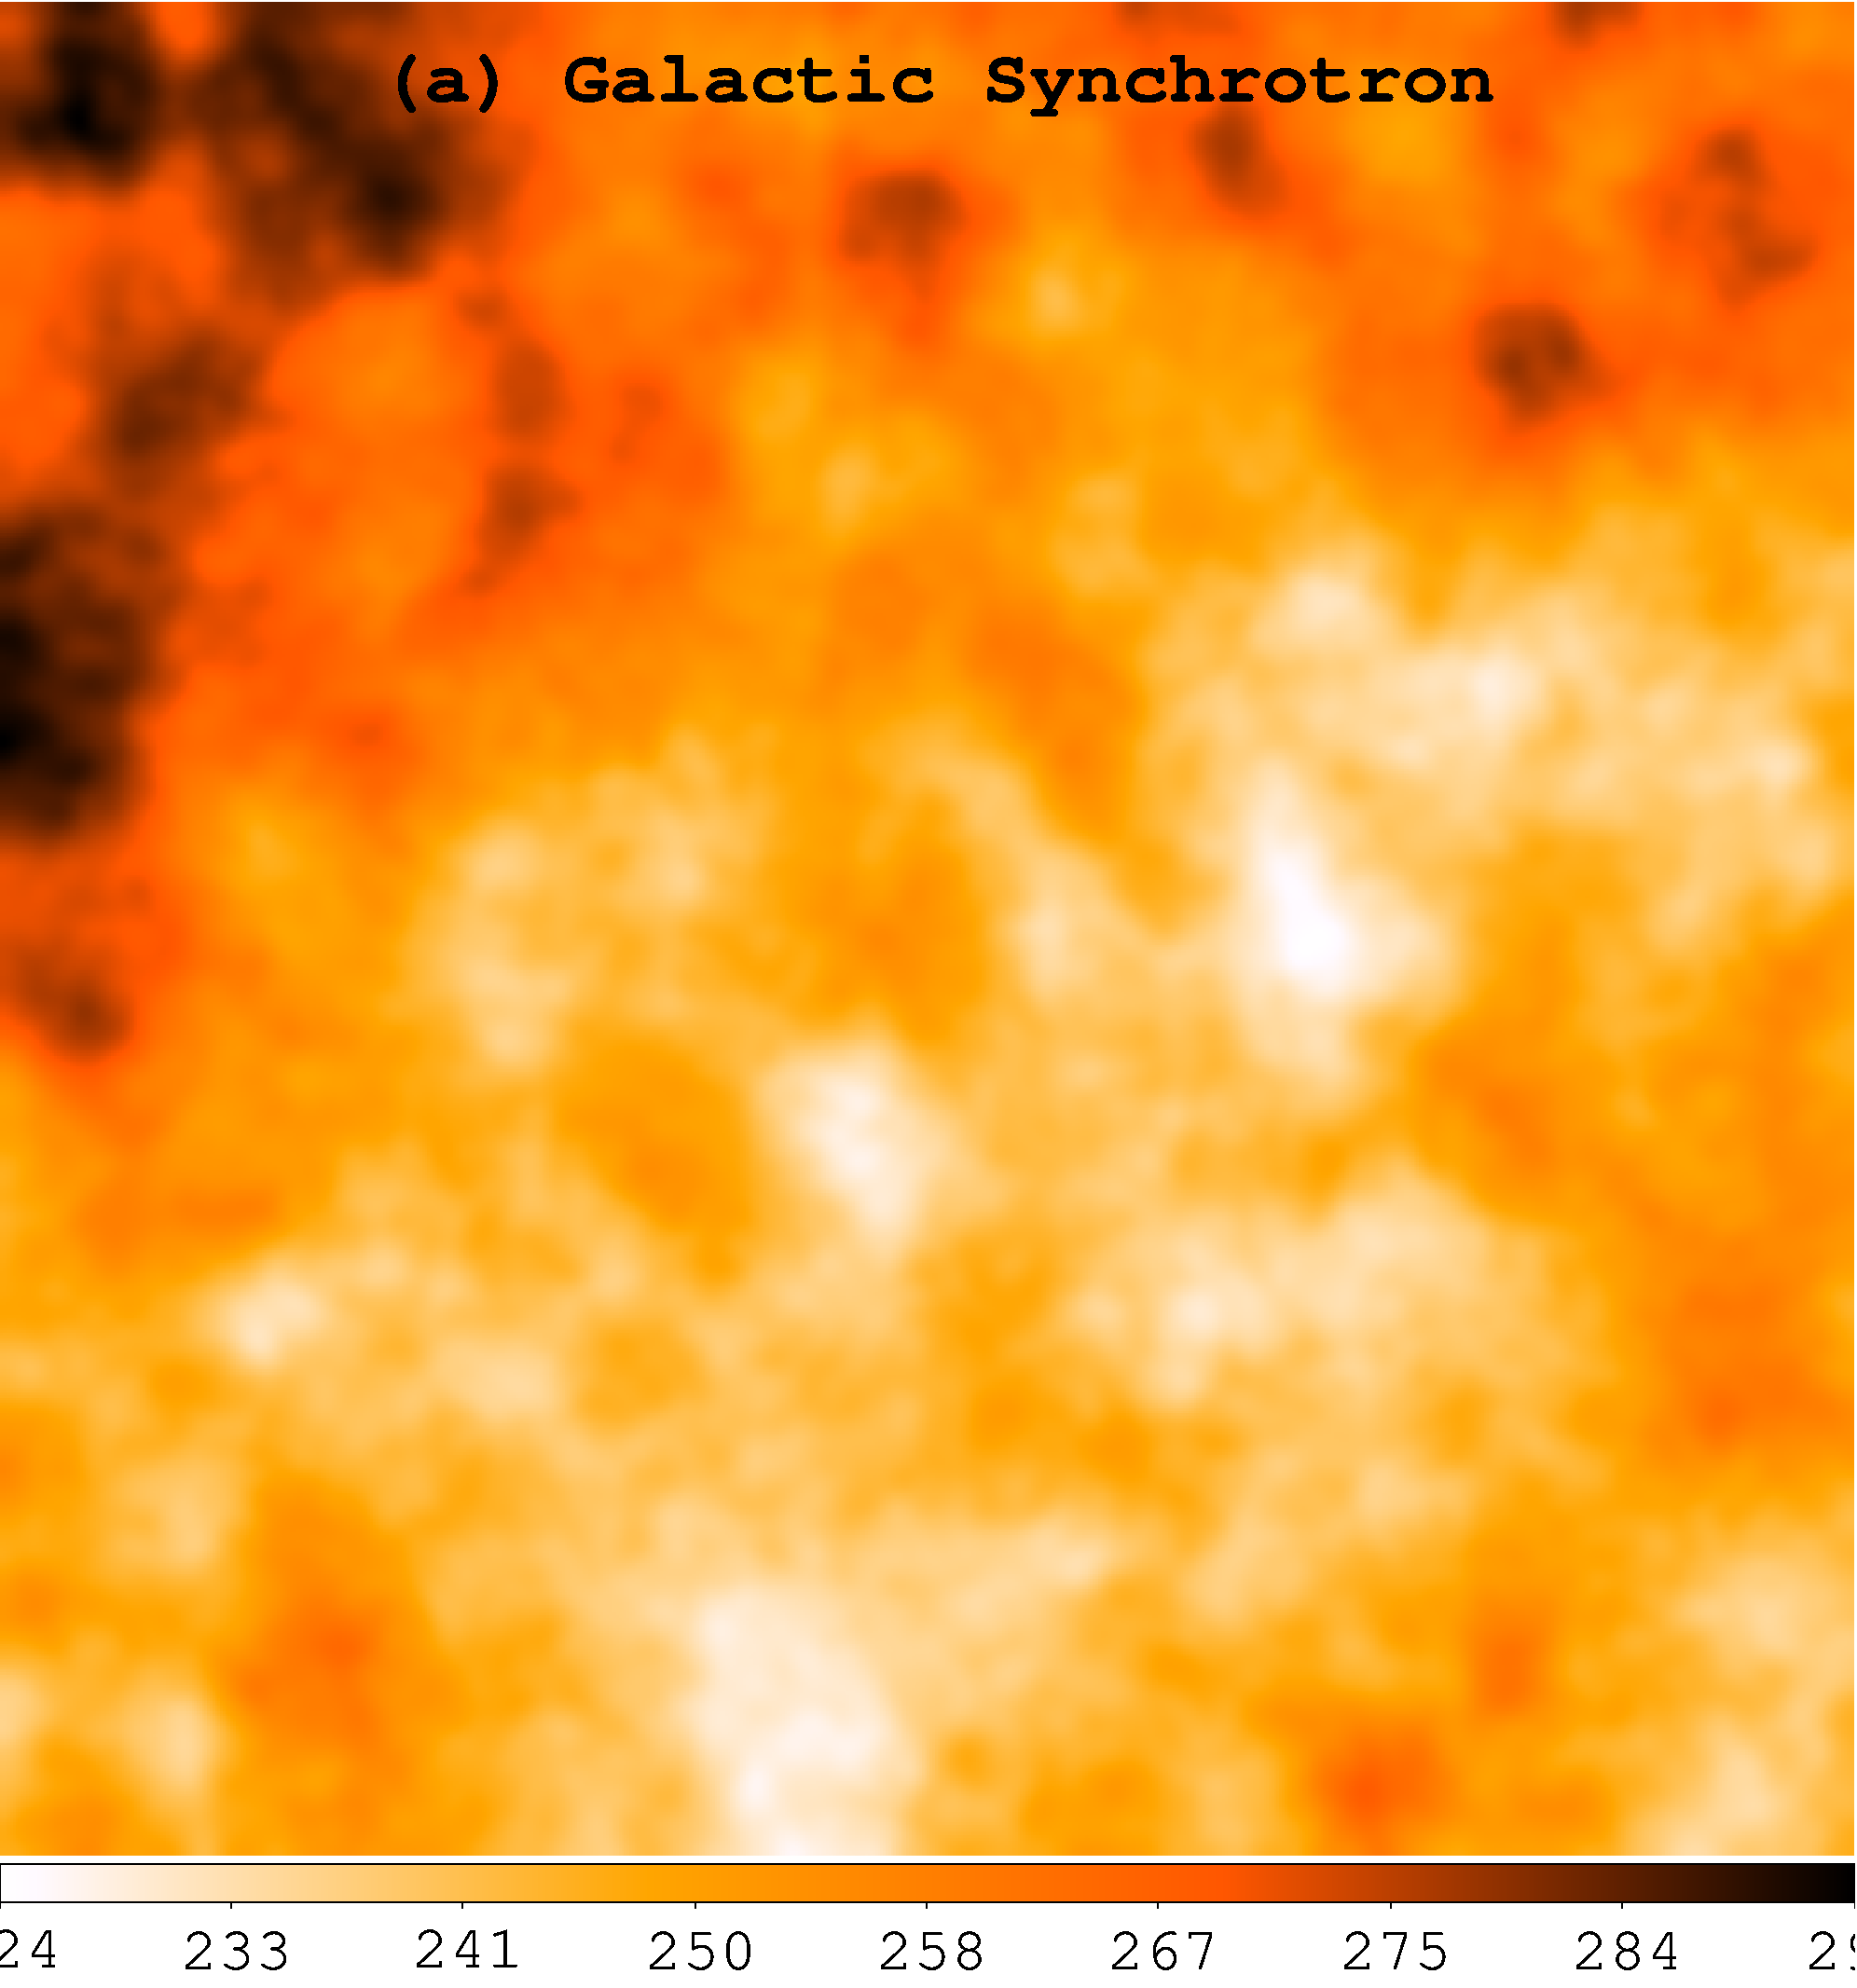
\includegraphics[width=0.32\textwidth]{gsyn-f158-heat}
  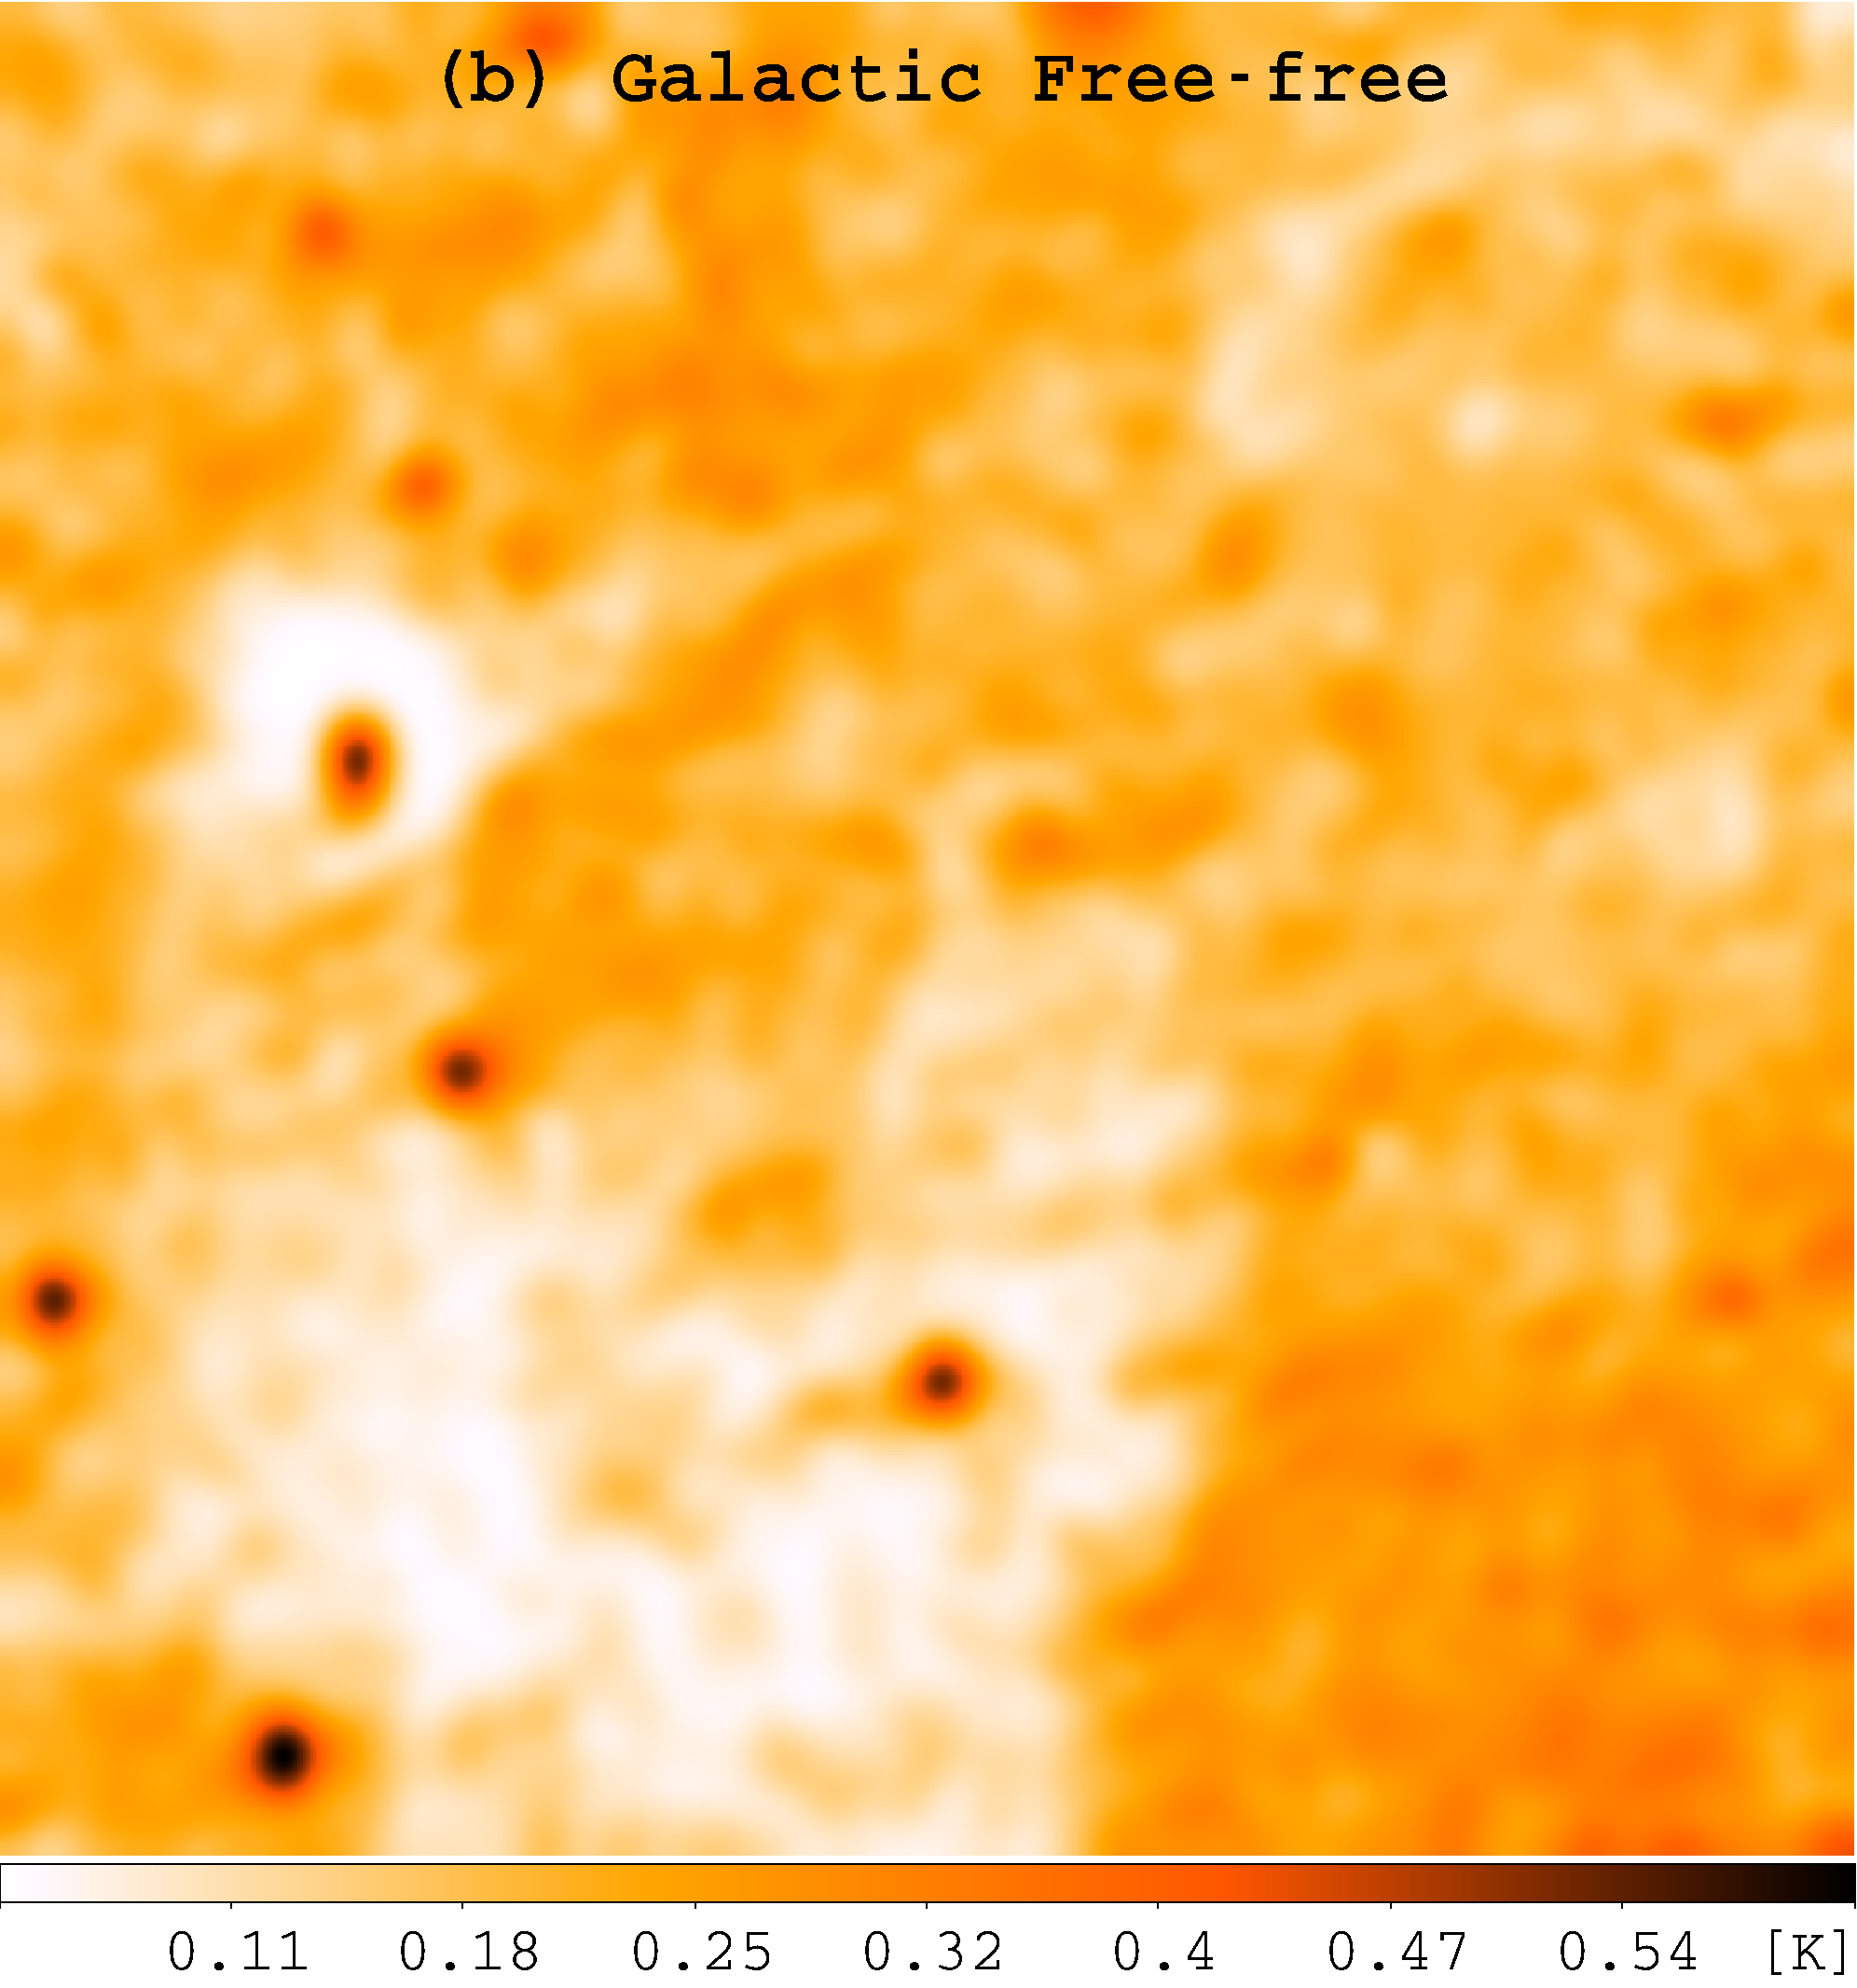
\includegraphics[width=0.32\textwidth]{gff-f158-heat}
  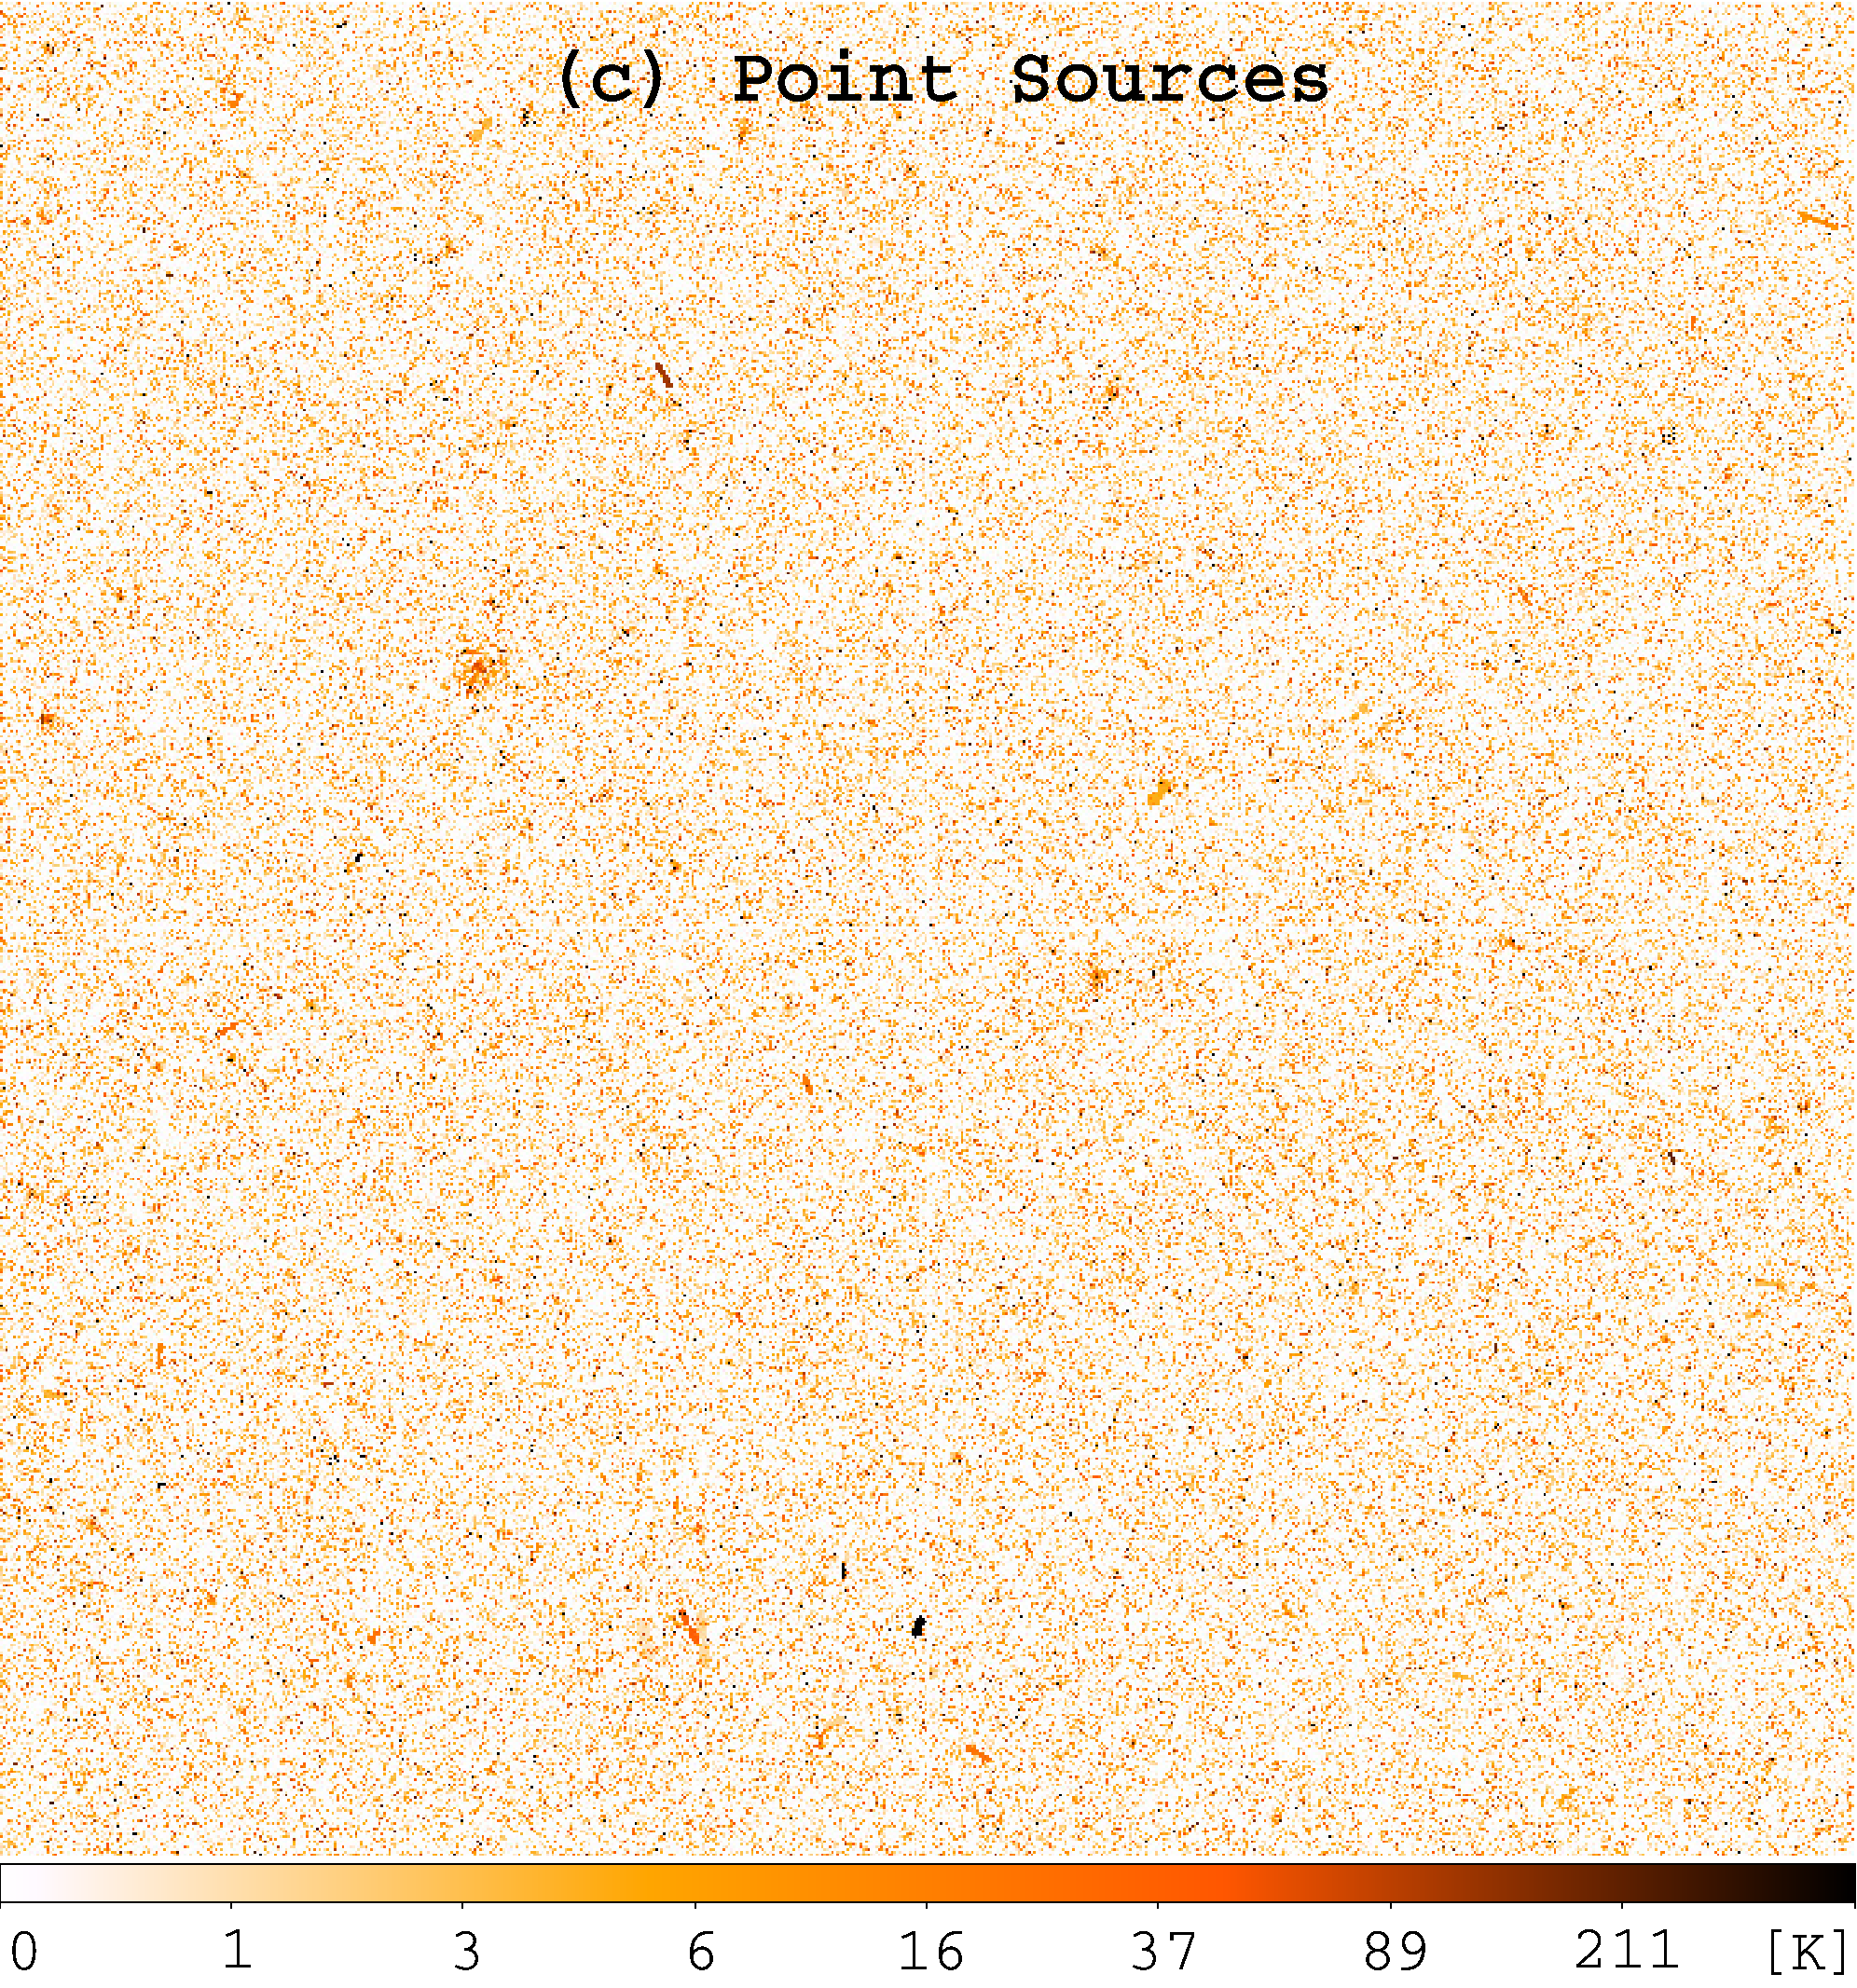
\includegraphics[width=0.32\textwidth]{pointsources-f158-heat-log}
  \caption{\label{fig:map-fg-other}%
    The sky maps of
    \textbf{(a)} the Galactic synchrotron emission,
    \textbf{(b)} the Galactic free-free emission, and
    \textbf{(c)} the extragalactic point sources
    at \SI{158}{\MHz}.
    All the maps cover sky region of size
    \SI[product-units=repeat]{10 x 10}{\degree},
    and have color bar in units of \si{\kelvin}.
  }
\end{figure*}


%========================================================================
\subsection{The EoR Signal}
\label{sec:eor-signal}
%========================================================================

The sky maps of the EoR signal are created using the 2016 data release
from the Evolution Of 21~cm Structure project\footnote{%
  Evolution Of 21~cm Structure project:
  \url{http://homepage.sns.it/mesinger/EOS.html}}.
The project used \texttt{21cmFAST} version 2 \citep{mesinger2011} to
simulate the cosmic reionization process from redshift 86.5 to 5.0 inside
a large cube which is 1.6 comoving \si{\Gpc} (1024 cells) along each side
\citep{mesinger2016}.
We extract the image slices at needed frequencies (i.e., redshifts) from
the light-cone cubes of the recommended \enquote{faint galaxies} case,
and then tile and re-scale them to have the same sky coverage and
pixel size as our foreground maps.
\autoref{fig:eor-tbrms} shows the \rms{} brightness temperatures of the
EoR signal among \SIrange{120}{200}{\MHz} ($z = \numrange{6.1}{10.8}$).
The corresponding \rms{} brightness temperatures at the central
frequencies of the three adopted bands and the map of the EoR signal
obtained at \SI{158}{\MHz} are given in \autoref{tab:tb-rms} and
\autoref{fig:map-eor}, respectively.

\begin{figure}
  \centering
  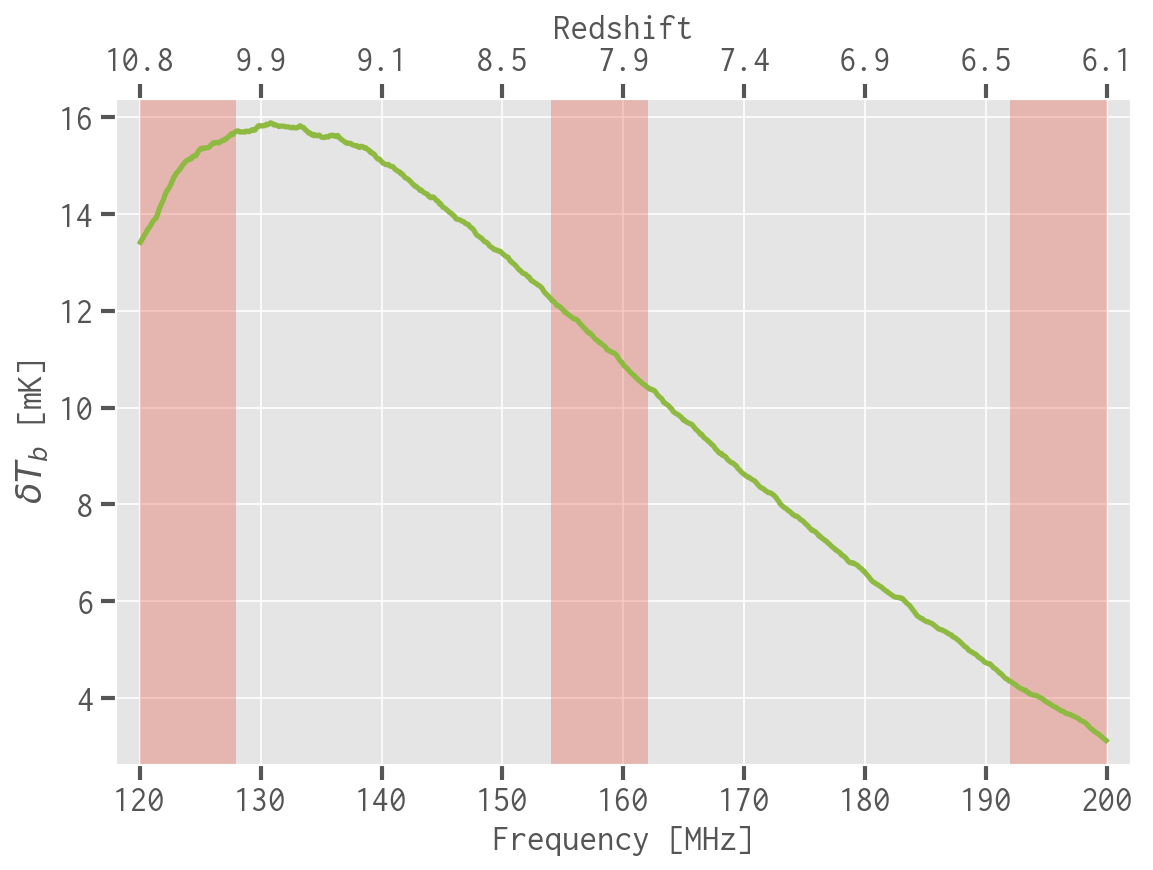
\includegraphics[width=0.7\textwidth]{eos2016-tbrms}
  \caption{\label{fig:eor-tbrms}%
    The \rms{} brightness temperatures of the EoR signal
    (green solid line) within \SIrange{120}{200}{\MHz}
    ($z = \numrange{6.1}{10.8}$).
    The red shaded regions mark the \numrange{120}{128},
    \numrange{154}{162}, and \numrange{192}{200} \si{\MHz}
    frequency bands adopted in this work.
  }
\end{figure}

\begin{figure}
  \centering
  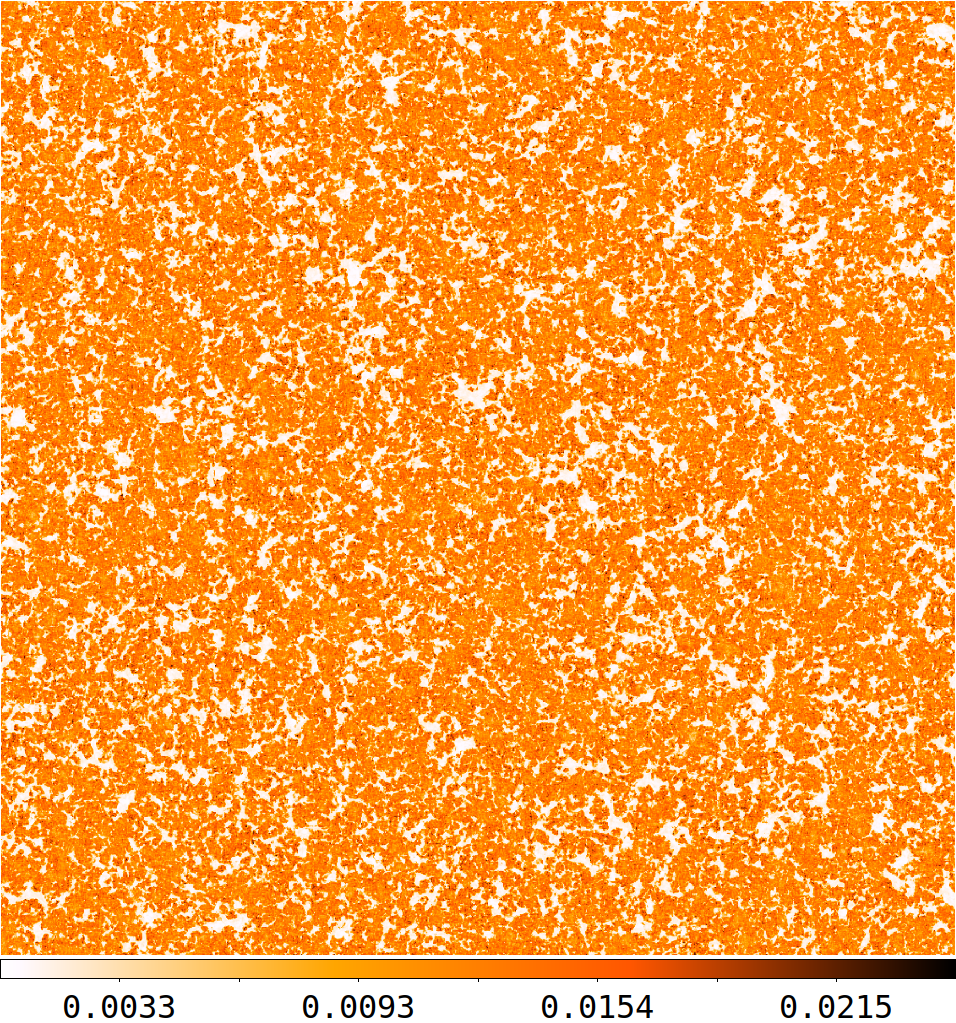
\includegraphics[width=0.6\textwidth]{21cm-f158-heat2}
  \caption{\label{fig:map-eor}%
    The sky map of the EoR signal at \SI{158}{\MHz}.
    The sky region size is \SI[product-units=repeat]{10 x 10}{\degree},
    and the color bar is in units of \si{\kelvin}.
  }
\end{figure}


%########################################################################
\section{Simulated SKA Observations}
\label{sec:obs-simu}
%########################################################################

In order to properly evaluate the contamination caused by radio halos
on the EoR observations, it is essential to take account of the
practical instrumental effects of radio interferometers.
Therefore, we employ the latest SKA1-Low layout configuration\footnote{%
  SKA1-Low Configuration Coordinates:
  \url{https://astronomers.skatelescope.org/wp-content/uploads/2016/09/SKA-TEL-SKO-0000422_02_SKA1_LowConfigurationCoordinates-1.pdf}
  (released on 2016 May 21)
}
to simulate the \enquote{observed} images of the above simulated sky maps.
According to the layout configuration,
the SKA1-Low interferometer consists of 512 stations, with 224 of them
randomly distributed within the \enquote{core} of \SI{1000}{\meter} in
diameter, while the remaining stations are grouped into \enquote{clusters}
and placed on 3 spiral arms extending up to a radius of
\SI{\sim 35}{\kilo\meter}.
Each station has 256 antennas randomly distributed with a minimum separation
of $d_{\R{min}} = \SI{1.5}{\meter}$ inside a circular region of
\SI{35}{\meter} in diameter \citep[e.g.,][]{mort2017}.
With this layout configuration, the dense core makes the SKA1-Low very
sensitive to the EoR signal, while the long baselines greatly help the
foreground characterization and removal, as well as other scientific goals.

The \SI{8}{\MHz} bandwidth of each frequency band is divided into 51
channels for a frequency resolution of \SI{160}{\kilo\hertz}.
For each component, we simulate the input sky maps at every frequency
channel by following the steps described in \autoref{sec:sky-simu},
and then use the \texttt{OSKAR}\footnote{%
  OSKAR: \url{https://github.com/OxfordSKA/OSKAR} (version 2.7.0)}
simulator \citep{mort2010} to perform observations
for \SI{6}{\hour} ($\pm \SI{3}{\hour}$ in Hour Angle) with the
SKA1-Low layout configuration.
{\color{cyan}%
The input sky maps are centered at sky position of
(R.A., Dec.)\ = (\SI{0}{\degree}, \SI{-27}{\degree}),
which passes through the zenith of the SKA1-Low telescope and
is an ideal choice for the simulated observations.}
The simulated visibility data are imaged through the
\texttt{WSClean}\footnote{%
  WSClean: \url{https://sourceforge.net/p/wsclean} (version 2.5)}
imager \citep{offringa2014} using Briggs' weighting with a
robustness of zero \citep{briggs1995},
and the created images are cropped to keep only the central regions
because the marginal regions suffer from the problem of insufficient
CLEAN.
As the telescope's field of view (\fov) is inversely proportional to
the observing frequency, we choose to keep the central
\SI[product-units=repeat]{6 x 6}{\degree},
\SI[product-units=repeat]{5 x 5}{\degree}, and
\SI[product-units=repeat]{4 x 4}{\degree}
regions in the \numrange{120}{128}, \numrange{154}{162}, and
\numrange{192}{200} \si{\MHz} frequency bands, respectively.

Since Galactic synchrotron and free-free emissions have similar
diffuse features, they are combined for the simulated observations.
Similar to the real-time peeling of the brightest point sources in
practical data analysis pipelines
\citep[e.g.,][]{mitchell2008,intema2009,mort2017},
we assume that the point sources with a \SI{158}{\MHz} flux density
$S_{158} > \SI{50}{\mJy}$ are removed \citep[e.g.,][]{pindor2011}.
The \rms{} brightness temperatures of extragalactic point sources are
hence significantly reduced to be about
\SIlist[%
  list-units=brackets,
  scientific-notation=fixed,
  fixed-exponent=4,
]{22.5e4;9.81e4;4.75e4}{\mK}
at \numlist{124;158;196} \si{\MHz}, respectively.
Moreover, we create the foreground image cubes in each frequency band
using the CLEAN algorithm with joined-channel deconvolution in order
to ensure the spectral smoothness \citep{offringa2017}, which is
crucial to extract the EoR signal from the overwhelming foregrounds.
For the EoR signal, we directly use the dirty images because the CLEAN
algorithm is not well applicable to such faint and diffuse emissions.
Hence we obtain the \enquote{observed} image cubes of the EoR signal,
radio halos, the Galactic diffuse emission (with both synchrotron and
free-free emission), and the extragalactic point sources (with the
brightest ones removed) in the \numrange{120}{128}, \numrange{154}{162},
and \numrange{192}{200} \si{\MHz} frequency bands.


%########################################################################
\section{Power Spectra and EoR Window}
\label{sec:ps-eorw}
%########################################################################

The redshifted 21~cm signal expected to be observed at different
frequencies represents a three-dimensional (3D) data cube, where the
two spatial dimensions describe the transverse distances across the sky
and the frequency dimension maps to the line-of-sight distance.
Within a limited redshift range (e.g., $\Delta z \sim 0.5$, corresponding
to a frequency bandwidth of \SI{\sim 8}{\MHz} at \SI{158}{\MHz})
during the EoR, the evolution effect of the Universe is minor and the
\Hi{} distribution is believed to be isotropic.
The corresponding 3D power spectrum $P(k_x, k_y, k_z)$ of the EoR signal
should have spherical symmetry and can be averaged in spherical shells
of radii $k$, yielding the one-dimensional (1D) power spectrum $P(k)$,
which effectively increases the signal-to-noise ratio compared to
direct imaging observations \citep{morales2004,morales2006,datta2010}.
The \enquote{dimensionless} variant of the 1D power spectrum
$\Delta^2(k) = P(k) \,k^3 / (2\pi^2)$
is more commonly used in the literature.
To suppress the significant side-lobes in the Fourier transform caused
by the sharp discontinuities at the ends of the finite frequency band,
we apply the Blackman-Nuttall window function to the frequency dimension
before calculating the power spectra \citep[e.g.,][]{trott2015,chapman2016}.

Since the two angular dimensions and the frequency dimension of the image
cubes of foreground continuum emissions are independent, which is
different from the image cube of the redshifted 21~cm signal, it is
appropriate to average the 3D power spectrum $P(k_x, k_y, k_z)$
over angular annuli of radii $\kperp \equiv \sqrt{k_x^2 + k_y^2}$
for each line-of-sight plane $\klos \equiv k_z$, which yields the
two-dimensional (2D) power spectrum $P(\kperp, \klos)$.
In the $(\kperp, \klos)$ plane, the spectral-smooth foreground emissions
are supposed to reside in the low-\klos{} region, although complicated
instrumental and observational effects (e.g., chromatic primary beams,
calibration errors) can throw some of the foreground contamination from
the purely angular (\kperp) modes into the line-of-sight (\klos)
dimension (i.e., mode mixing), which results in an expanded wedge-like
contamination region at the bottom-right in the $(\kperp, \klos)$ plane
(\enquote{foreground wedge}; \citealt{datta2010,morales2012,liu2014}).
The region almost free of the foreground contamination, namely the
\enquote{EoR window,} is preserved at the top-left in the
$(\kperp, \klos)$ plane and can be characterized by \citep{thyagarajan2013}
\begin{equation}
  \label{eq:eor-window}
  \klos \geq \frac{H(z) D_{\!M}(z)}{c (1+z)} \left[
    \kperp \sin\Theta +
    \frac{e}{B} \frac{2\pi f_{21}}{(1+z) D_{\!M}(z)} \right],
\end{equation}
where
$c$ is the speed of light,
$B = \SI{8}{\MHz}$ is the frequency bandwidth of the image cube,
$f_{21} = \SI{1420.4}{\MHz}$ is the rest-frame frequency of the 21~cm line,
$z = f_{21}/f_c - 1$ is the signal redshift corresponding to the central
frequency ($f_c$) of the image cube,
$H(z)$ is the Hubble parameter at redshift $z$ [see \autoref{eq:hubble-z}],
$D_{\!M}(z)$ is the transverse comoving distance,
$e$ denotes the number of characteristic convolution widths
($\propto B^{-1}$) for the spillover region caused by the variations in
instrumental frequency response,
and $\Theta$ is the angular distance of foreground sources from the
field center.


%########################################################################
\section{Results}
\label{sec:results}
%########################################################################

The methods proposed to tackle the foreground contamination can be
classified into two broad categories: foreground removal and foreground
avoidance.
The former applies appropriate foreground models to directly subtract
the contamination, while the latter makes use of the 2D power spectra
and measures the EoR signal only inside the EoR window to avoid the
severe foreground contamination.
More details can be found in \citet[and references therein]{chapman2016}.
We evaluate how EoR measurements will be affected by radio halos in both
cases accordingly.
First, we calculate the 3D power spectra from the image cubes that are
obtained in the simulations in \autoref{sec:obs-simu}.
By averaging the 3D power spectra, we calculate the 1D power spectra
and compare the intensities of radio halos with the EoR signal, which
illustrates the impacts of radio halos on the EoR measurements with the
foreground removal methods.
Next, we calculate the 2D power spectra and carry out the comparison
between radio halos and the EoR signal inside the EoR window, from
which we evaluate the effects imposed by radio halos in adopting the
foreground avoidance methods to extract the EoR signal.


%========================================================================
\subsection{1D Power Spectra}
\label{sec:ps1d}
%========================================================================

\begin{figure*}
  \centering
  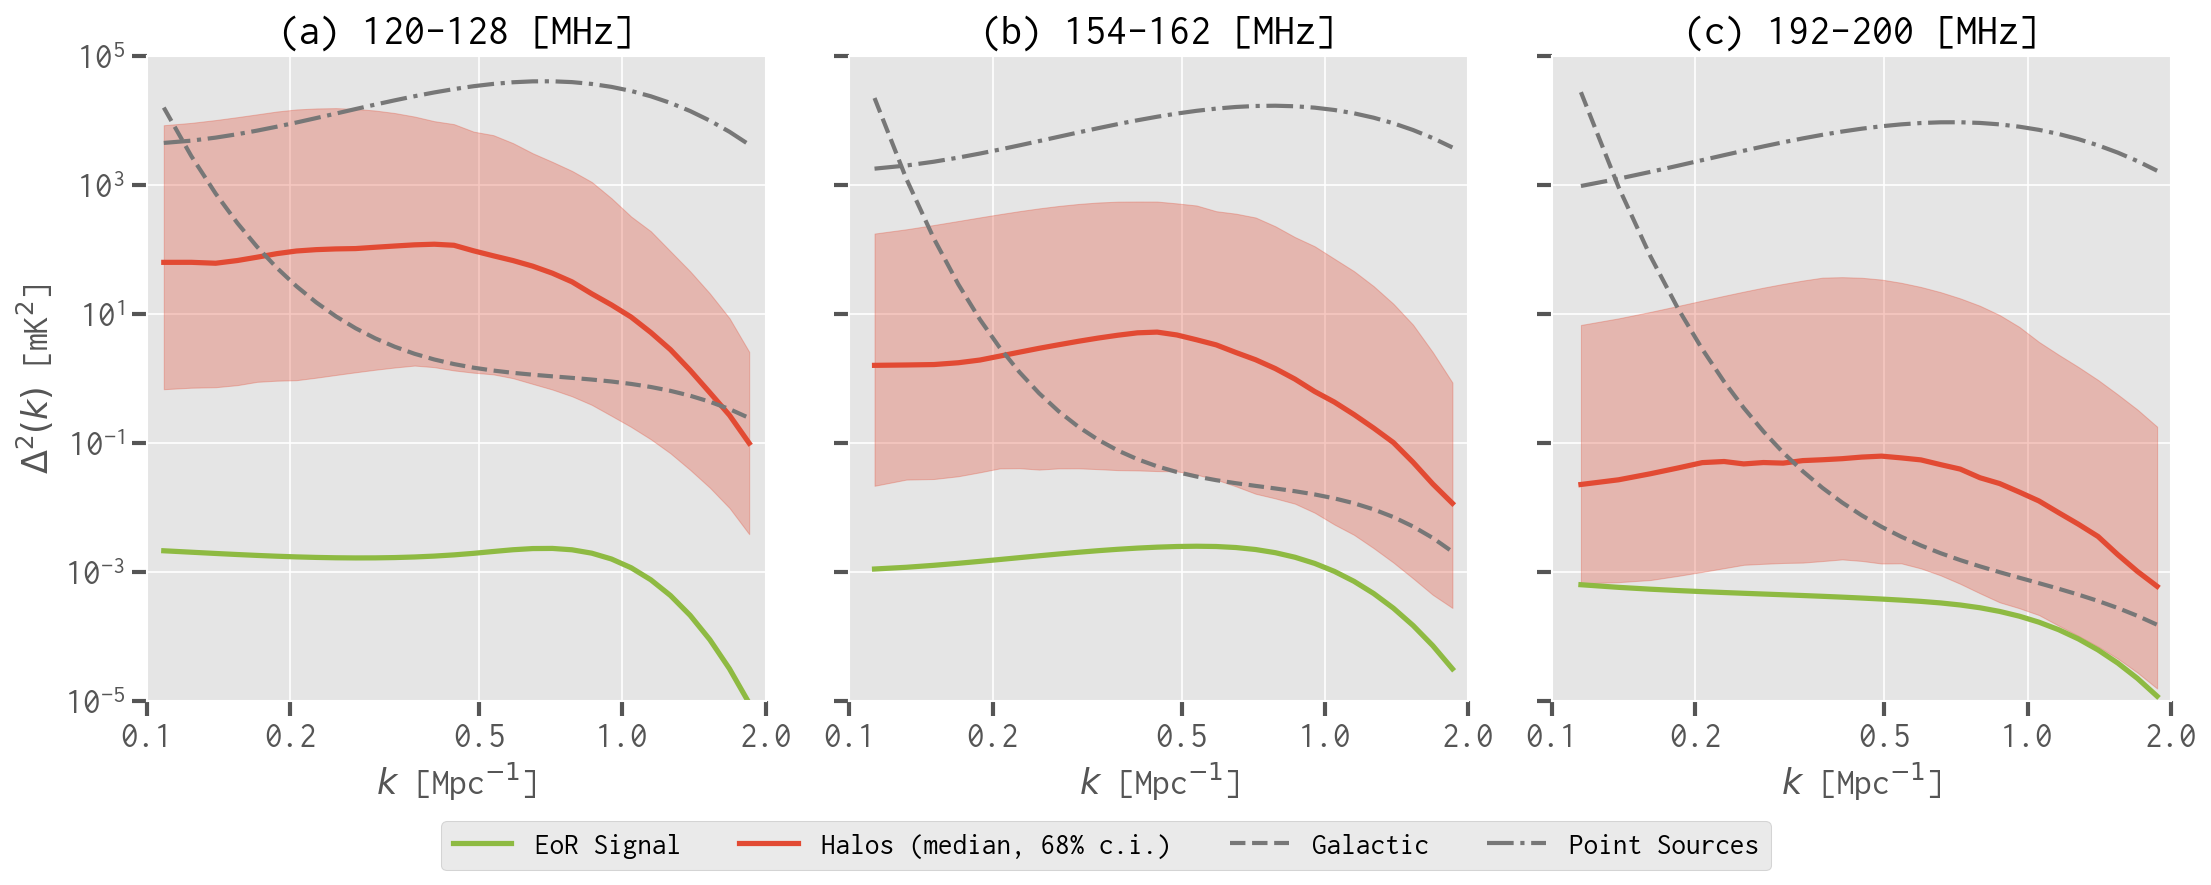
\includegraphics[width=\textwidth]{ps1d-3bands}
  \caption{\label{fig:ps1d-3bands}%
    Comparisons of the 1D dimensionless power spectra $\Delta^2(k)$
    among the EoR signal (green solid line), radio halos (red solid line),
    Galactic diffuse emission (gray dashed line), and extragalactic point
    sources (gray dash-dotted line) in the
    \textbf{(a)} \SIrange{120}{128}{\MHz},
    \textbf{(b)} \SIrange{154}{162}{\MHz}, and
    \textbf{(c)} \SIrange{192}{200}{\MHz} frequency bands.
    The red solid lines and shaded regions represent the median and the
    corresponding \SI{68}{\percent} confidence interval of the power
    spectra for radio halos estimated from the 100 simulation runs.
  }
\end{figure*}

We calculate the 1D dimensionless power spectra $\Delta^2(k)$ for each
image cube obtained in \autoref{sec:obs-simu}.
For radio halos, we utilize all the 100 simulation runs
(\autoref{sec:cluster-halos}) to estimate the median power spectra and
the corresponding \SI{68}{\percent} confidence intervals (c.i.\@) in each
frequency band.
The comparisons of the power spectra $\Delta^2(k)$ between radio halos
and the EoR signal in each frequency band are displayed
in \autoref{fig:ps1d-3bands}, where we also show the power spectra of
Galactic diffuse emission and extragalactic point sources for comparison.
The median power spectra (red solid lines) show that radio halos are
generally stronger than the EoR signal by about 4, 3, and 2 orders of
magnitude on the scales  of $\SI{0.1}{\per\Mpc} < k < \SI{2}{\per\Mpc}$
in the \numrange{120}{128}, \numrange{154}{162}, and \numrange{192}{200}
\si{\MHz} bands, respectively.
Given the large uncertainties in, e.g., brightness and number density, of
radio halos, the power spectra can vary by about \numrange{10}{100} times
with respect to the median values within the typical \SI{68}{\percent}
uncertainties (red shaded regions).
We also find that, although on large scales
($k \lesssim \SI{0.1}{\per\Mpc}$) the Galactic foreground is the
strongest contaminating source, its intensity deceases rapidly as the
scale becomes smaller.
On scales of $\SI{0.5}{\per\Mpc} \lesssim k \lesssim \SI{1}{\per\Mpc}$,
the contribution of the Galactic foreground is weaker than the median
intensity of radio halos by a factor of about \numrange{10}{100} in all
the three bands.
These results evidently show that radio halos are severe foreground
sources, and they must be carefully handled when employing the foreground
removal methods to extract the EoR signal.

%========================================================================
\subsection{2D Power Spectra}
\label{sec:ps2d}
%========================================================================

\begin{figure*}
  \centering
  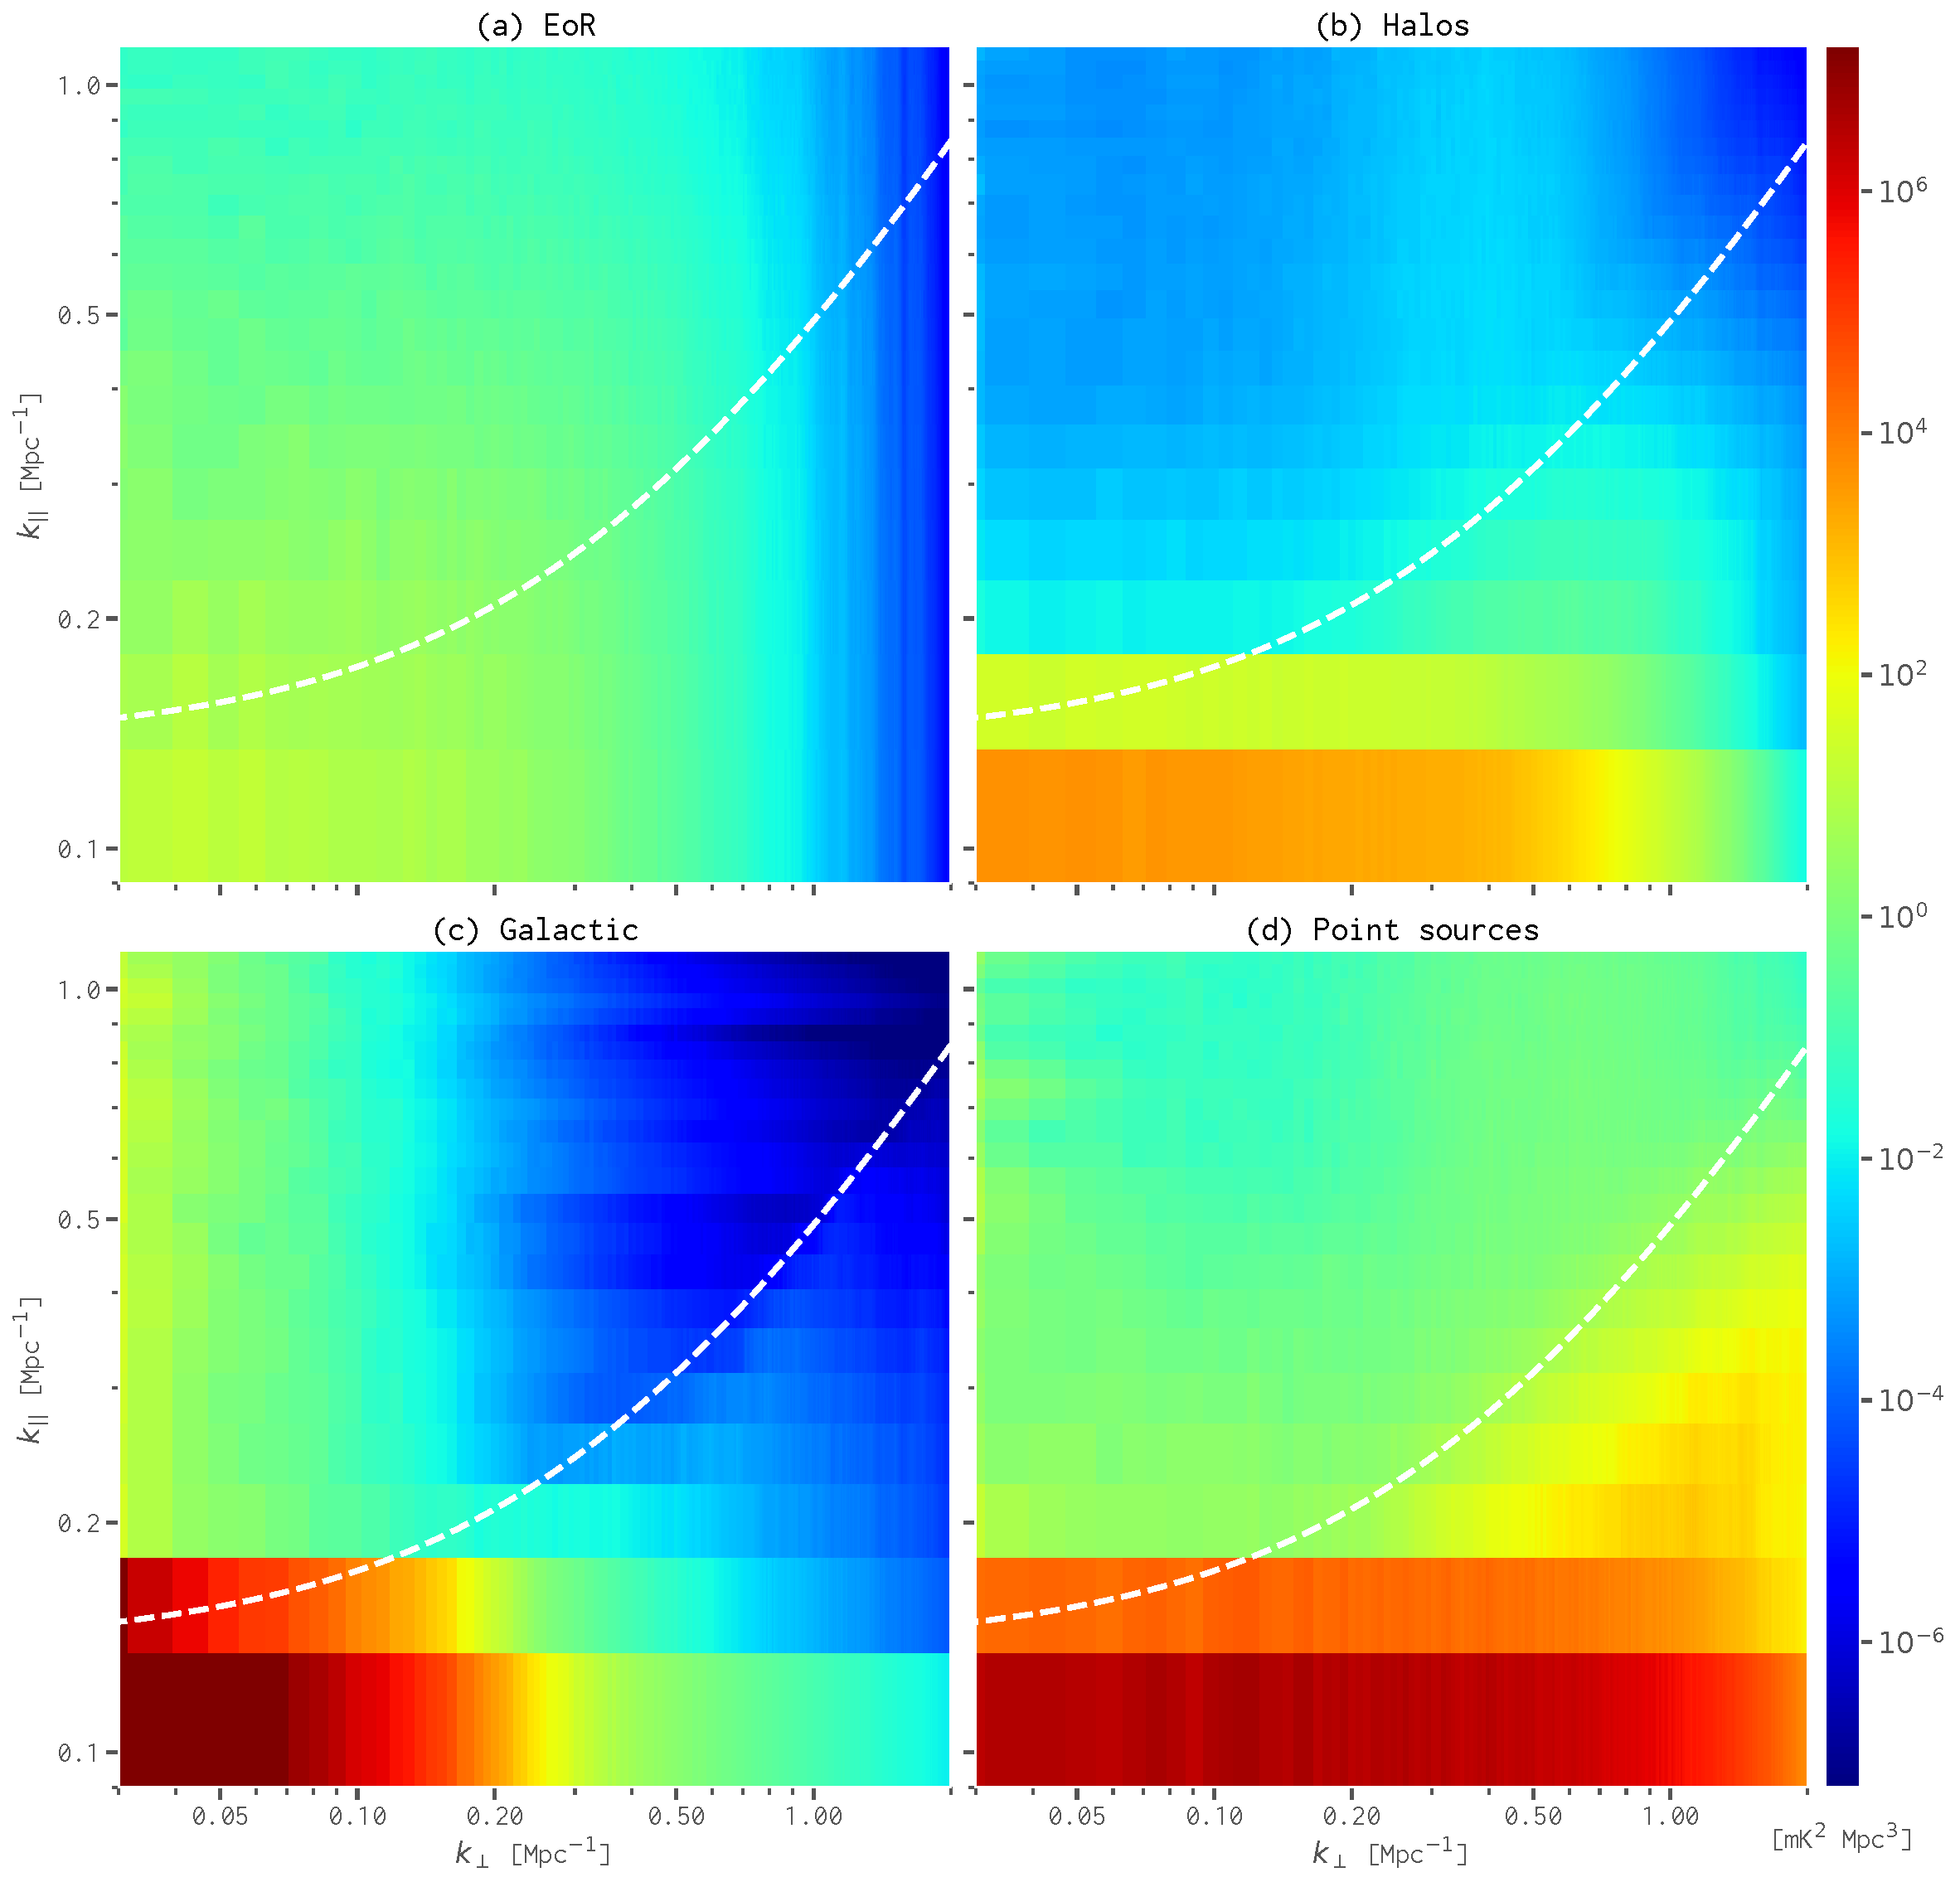
\includegraphics[width=0.8\textwidth]{ps2d-band158}
  \caption{\label{fig:ps2d}%
    The \SIrange{154}{162}{\MHz} 2D power spectra $P(\kperp, \klos)$ of
    \textbf{(a)} the EoR signal,
    \textbf{(b)} radio halos (median of the 100 simulation runs),
    \textbf{(c)} Galactic diffuse emission,
    and
    \textbf{(d)} extragalactic point sources.
    All panels share the same logarithmic scale in units of
    [\si{\mK\squared\Mpc\cubed}].
    The white dashed lines mark the boundary between the EoR window
    (at the top left) and the contaminating wedge (at the bottom right).
  }
\end{figure*}

In \autoref{fig:ps2d} we take the \SIrange{154}{162}{\MHz} band as an
example to show the 2D power spectra $P(\kperp, \klos)$ of the EoR signal,
radio halos (the median power spectrum of the 100 simulation runs),
Galactic diffuse emission, and extragalactic point sources.
We find that, as shown in many previous works,
the EoR signal distributes its power across all \klos{} modes,
illustrating its rapid fluctuations along the line-of-sight dimension,
while the spectral-smooth foreground components dominate only in the
low-\klos{} regions ($\klos{} \lesssim \SI{0.2}{\per\Mpc}$).
With regard to the angular dimension, the power of radio halos appears in
the range of $\kperp \lesssim \SI{1}{\per\Mpc}$, showing a concentration
on the intermediate scales of $\kperp \sim \SI{0.5}{\per\Mpc}$.
Meanwhile, the powers of Galactic diffuse emission and extragalactic
point sources dominate on the larger scales of
$\kperp \lesssim \SI{0.1}{\per\Mpc}$ and a broader angular scales of
$\kperp \gtrsim \SI{0.1}{\per\Mpc}$, respectively.
These results are also consistent with \autoref{fig:ps1d-3bands}(b).

\begin{figure*}
  \centering
  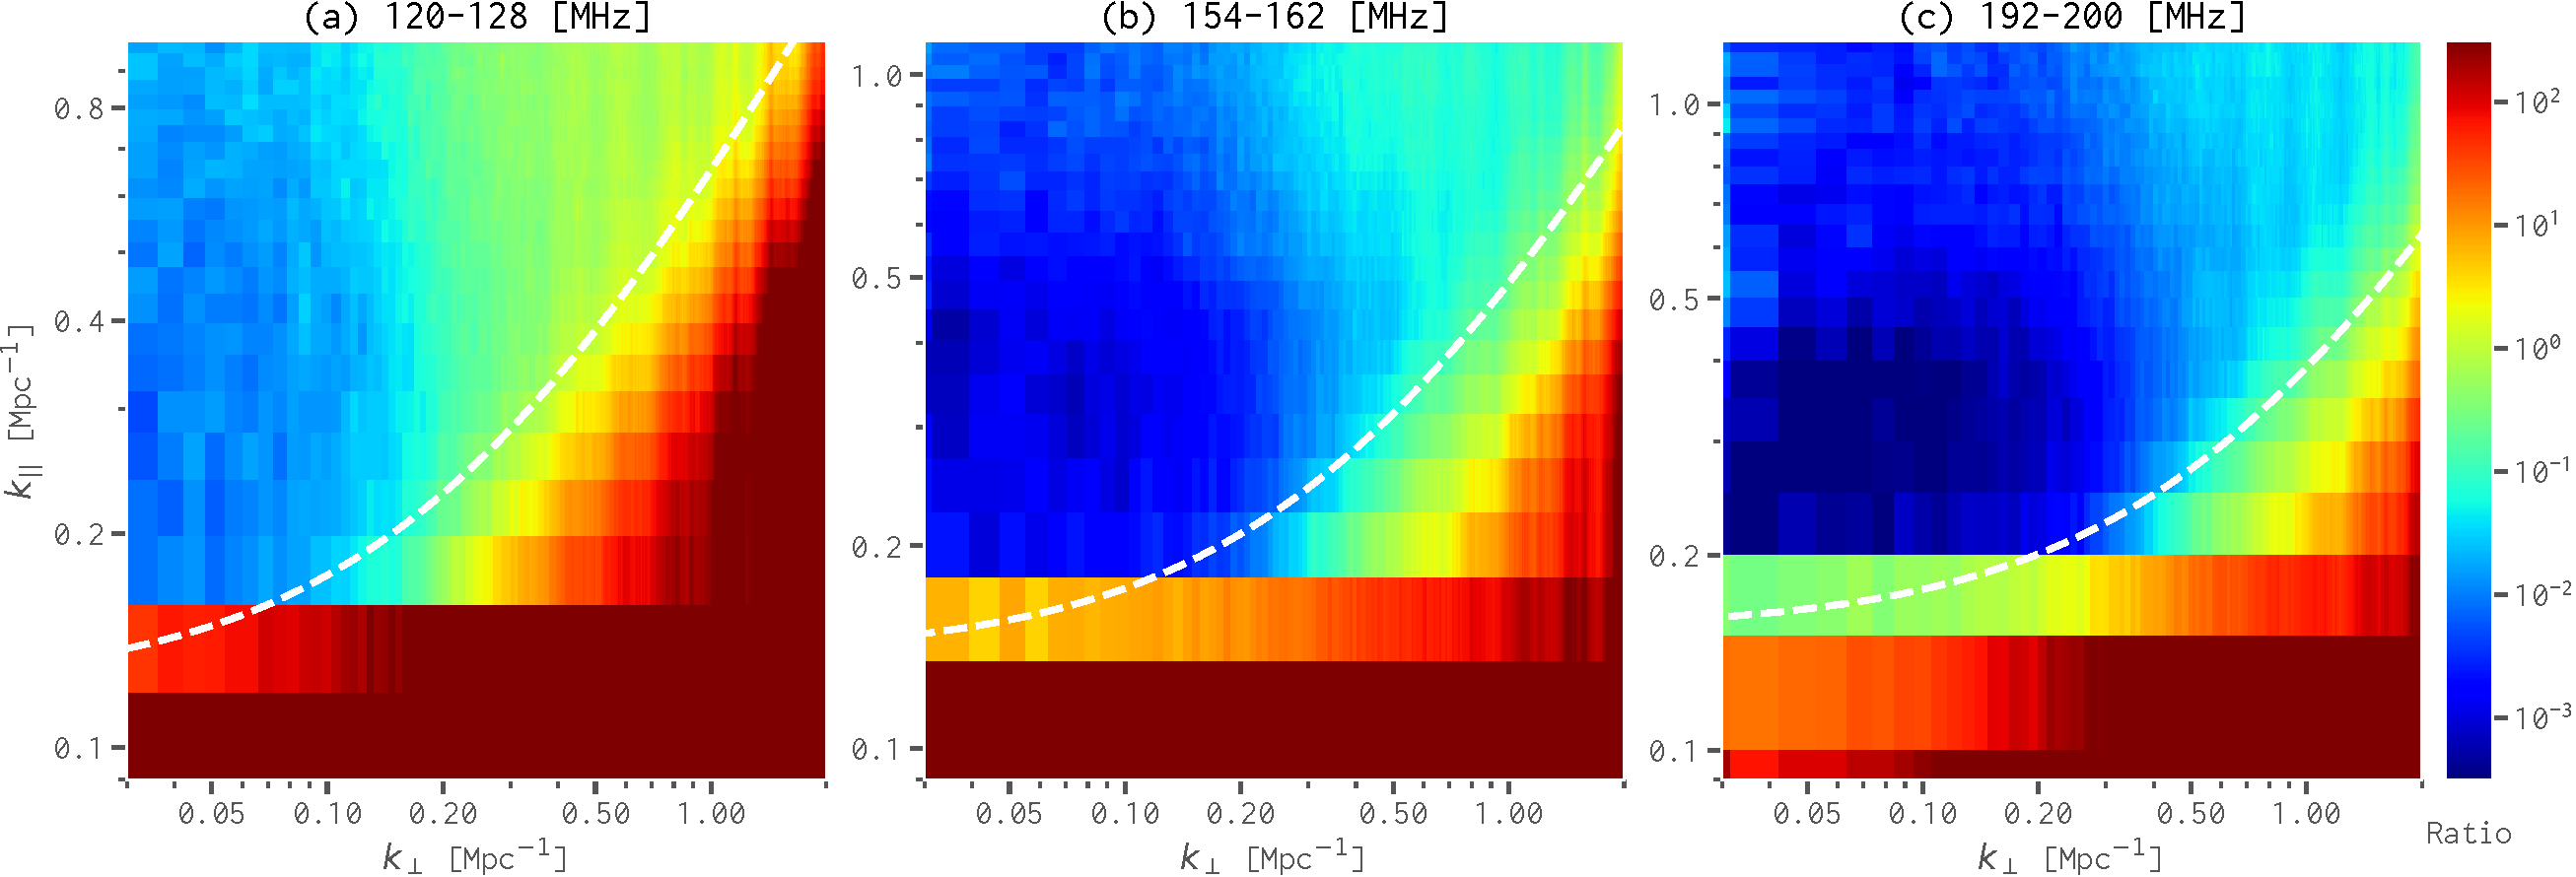
\includegraphics[width=\textwidth]{ps2d-ratio-3bands}
  \caption{\label{fig:ps2d-ratio}%
    2D power spectrum ratios $R(\kperp, \klos)$ of radio halos to the
    EoR signal in the
    \textbf{(a)} \SIrange{120}{128}{\MHz},
    \textbf{(b)} \SIrange{154}{162}{\MHz}, and
    \textbf{(c)} \SIrange{192}{200}{\MHz} frequency bands.
    The median 2D power spectrum of 100 simulation runs for radio halos
    is used.
    All panels use the same color bar with logarithmic scale.
    The white dashed lines mark the EoR window boundaries.
  }
\end{figure*}

In order to better evaluate the importance of radio halos as foreground
contaminating sources, we calculate the 2D power spectrum ratios
$R(\kperp, \klos)$ that are obtained by dividing the median 2D power
spectra of radio halos by those of the EoR signal in each frequency band,
and the results are presented in \autoref{fig:ps2d-ratio}.
We find that the EoR measurements will be significantly affected by radio
halos on angular scales of $\gtrsim \SI{0.1}{\per\Mpc}$,
$\gtrsim \SI{0.3}{\per\Mpc}$, and $\gtrsim \SI{0.5}{\per\Mpc}$ in the
\numrange{120}{128}, \numrange{154}{162}, and \numrange{192}{200}
\si{\MHz} bands, respectively.
It is also clearly shown that radio halos turn to cause stronger
contamination at lower frequencies (\SI{\sim 120}{\MHz}) than at higher
frequencies (\SI{\sim 200}{\MHz}).

\begin{figure}
  \centering
  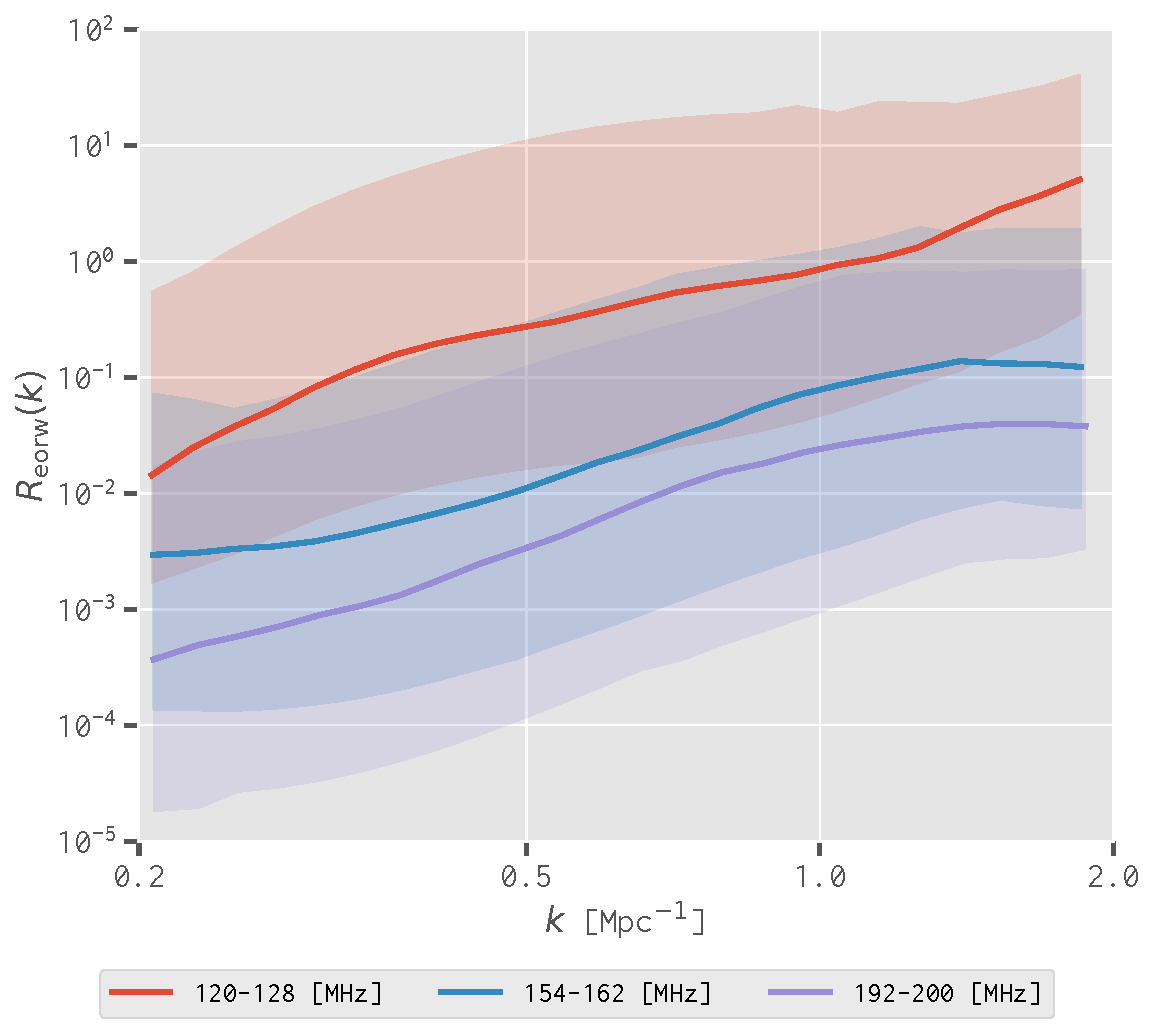
\includegraphics[width=0.6\textwidth]{ps1d-ratio-3bands}
  \caption{\label{fig:ps1d-ratio}%
    1D power ratios $R_{\R{eorw}}(k)$ inside the EoR window between
    radio halos to the EoR signal.
    The solid lines and shaded regions show the median and
    corresponding \SI{68}{\percent} uncertainties, respectively.
  }
\end{figure}

{\color{cyan}%
To further quantify the contamination caused by radio halos when
foreground avoidance methods are applied, we need to determine an EoR
window in the $(\kperp, \klos)$ plane that avoids the strong foreground
contamination and then compare the powers of radio halos and the EoR
signal inside the window.}
We have tested multiple parameter configurations ($e$, $\Theta$) as
defined in \autoref{eq:eor-window}, and find that when $e = 3$ and
$\Theta$ that is about 3 times the radius of SKA1-Low's \fov{} (i.e.,
$\Theta = \SI{7.5}{\degree}$, \SI{6.0}{\degree}, and \SI{4.8}{\degree}
in \numrange{120}{128}, \numrange{154}{162}, and \numrange{192}{200}
\si{\MHz}, respectively) are used, a conservative EoR window boundary
can be defined to effectively avoid the contaminating wedge
(Figures~\ref{fig:ps2d} and \ref{fig:ps2d-ratio}).
However, a significant part (about \SI{55}{\percent}, \SI{54}{\percent},
and \SI{40}{\percent} in the \numrange{120}{128}, \numrange{154}{162},
and \numrange{192}{200} \si{\MHz} bands, respectively) of the power of
the EoR signal is lost by adopting such EoR window boundaries.
By averaging the modes only inside the defined EoR window, we calculate
the 1D power spectrum ratios $R_{\R{eorw}}(k)$ of radio halos to the EoR
signal and present the results in the three frequency bands in
\autoref{fig:ps1d-ratio}.
We find that, on the scales of
$\SI{0.5}{\per\Mpc} \lesssim k \lesssim \SI{1.0}{\per\Mpc}$,
the 1D power ratios can be up to about
\SIrange[range-units=repeat]{1000}{2000}{\percent} in
\SIrange{120}{128}{\MHz},
\SIrange[range-units=repeat]{30}{100}{\percent} in
\SIrange{154}{162}{\MHz}, and
\SIrange[range-units=repeat]{10}{80}{\percent} in
\SIrange{192}{200}{\MHz}
within the \SI{68}{\percent} error bars (shaded regions).

Based on the above results, we conclude that radio halos are severe
foreground sources to the EoR observations at \SI{\sim 200}{\MHz}
and become much stronger contaminating sources at \SI{\sim 120}{\MHz}.
Even if inside the EoR window where most of the strong foreground
contamination is effectively avoided, radio halos can imprint
non-negligible contamination on the EoR measurements, especially at
lower frequencies (\SI{\sim 120}{\MHz}).


%########################################################################
\section{Discussions}
\label{sec:discussions}
%########################################################################

In practical observations with low-frequency radio interferometers, the
situations are much more complicated than our simulations.
For example, calibration uncertainties (e.g., insufficient sky modeling)
as well as other complicated instrumental and observational effects
(e.g., cable signal reflections, ionospheric distortions) can cause
frequency artifacts in the derived image cubes.
Foreground sources located in the side-lobes of the station beam can
also significantly reduce the imaging dynamical range and quality.
In this section, we investigate how the EoR measurements are affected
in these two situations if the contamination of radio halos is not
properly removed.

%========================================================================
\subsection{Instrumental Frequency Artifacts}
\label{sec:freq-artifacts}
%========================================================================

The smoothness along the frequency dimension is the most crucial feature
of various foreground components and is the key that enables us to
extract the faint EoR signal in the presence of overwhelming foreground
contamination.
However, artificial frequency structures may present in the obtained
image cubes due to calibration uncertainties and various instrumental
and observational effects, which break the spectral smoothness of the
foreground emission and hence damage the EoR measurements.

\begin{figure*}
  \centering
  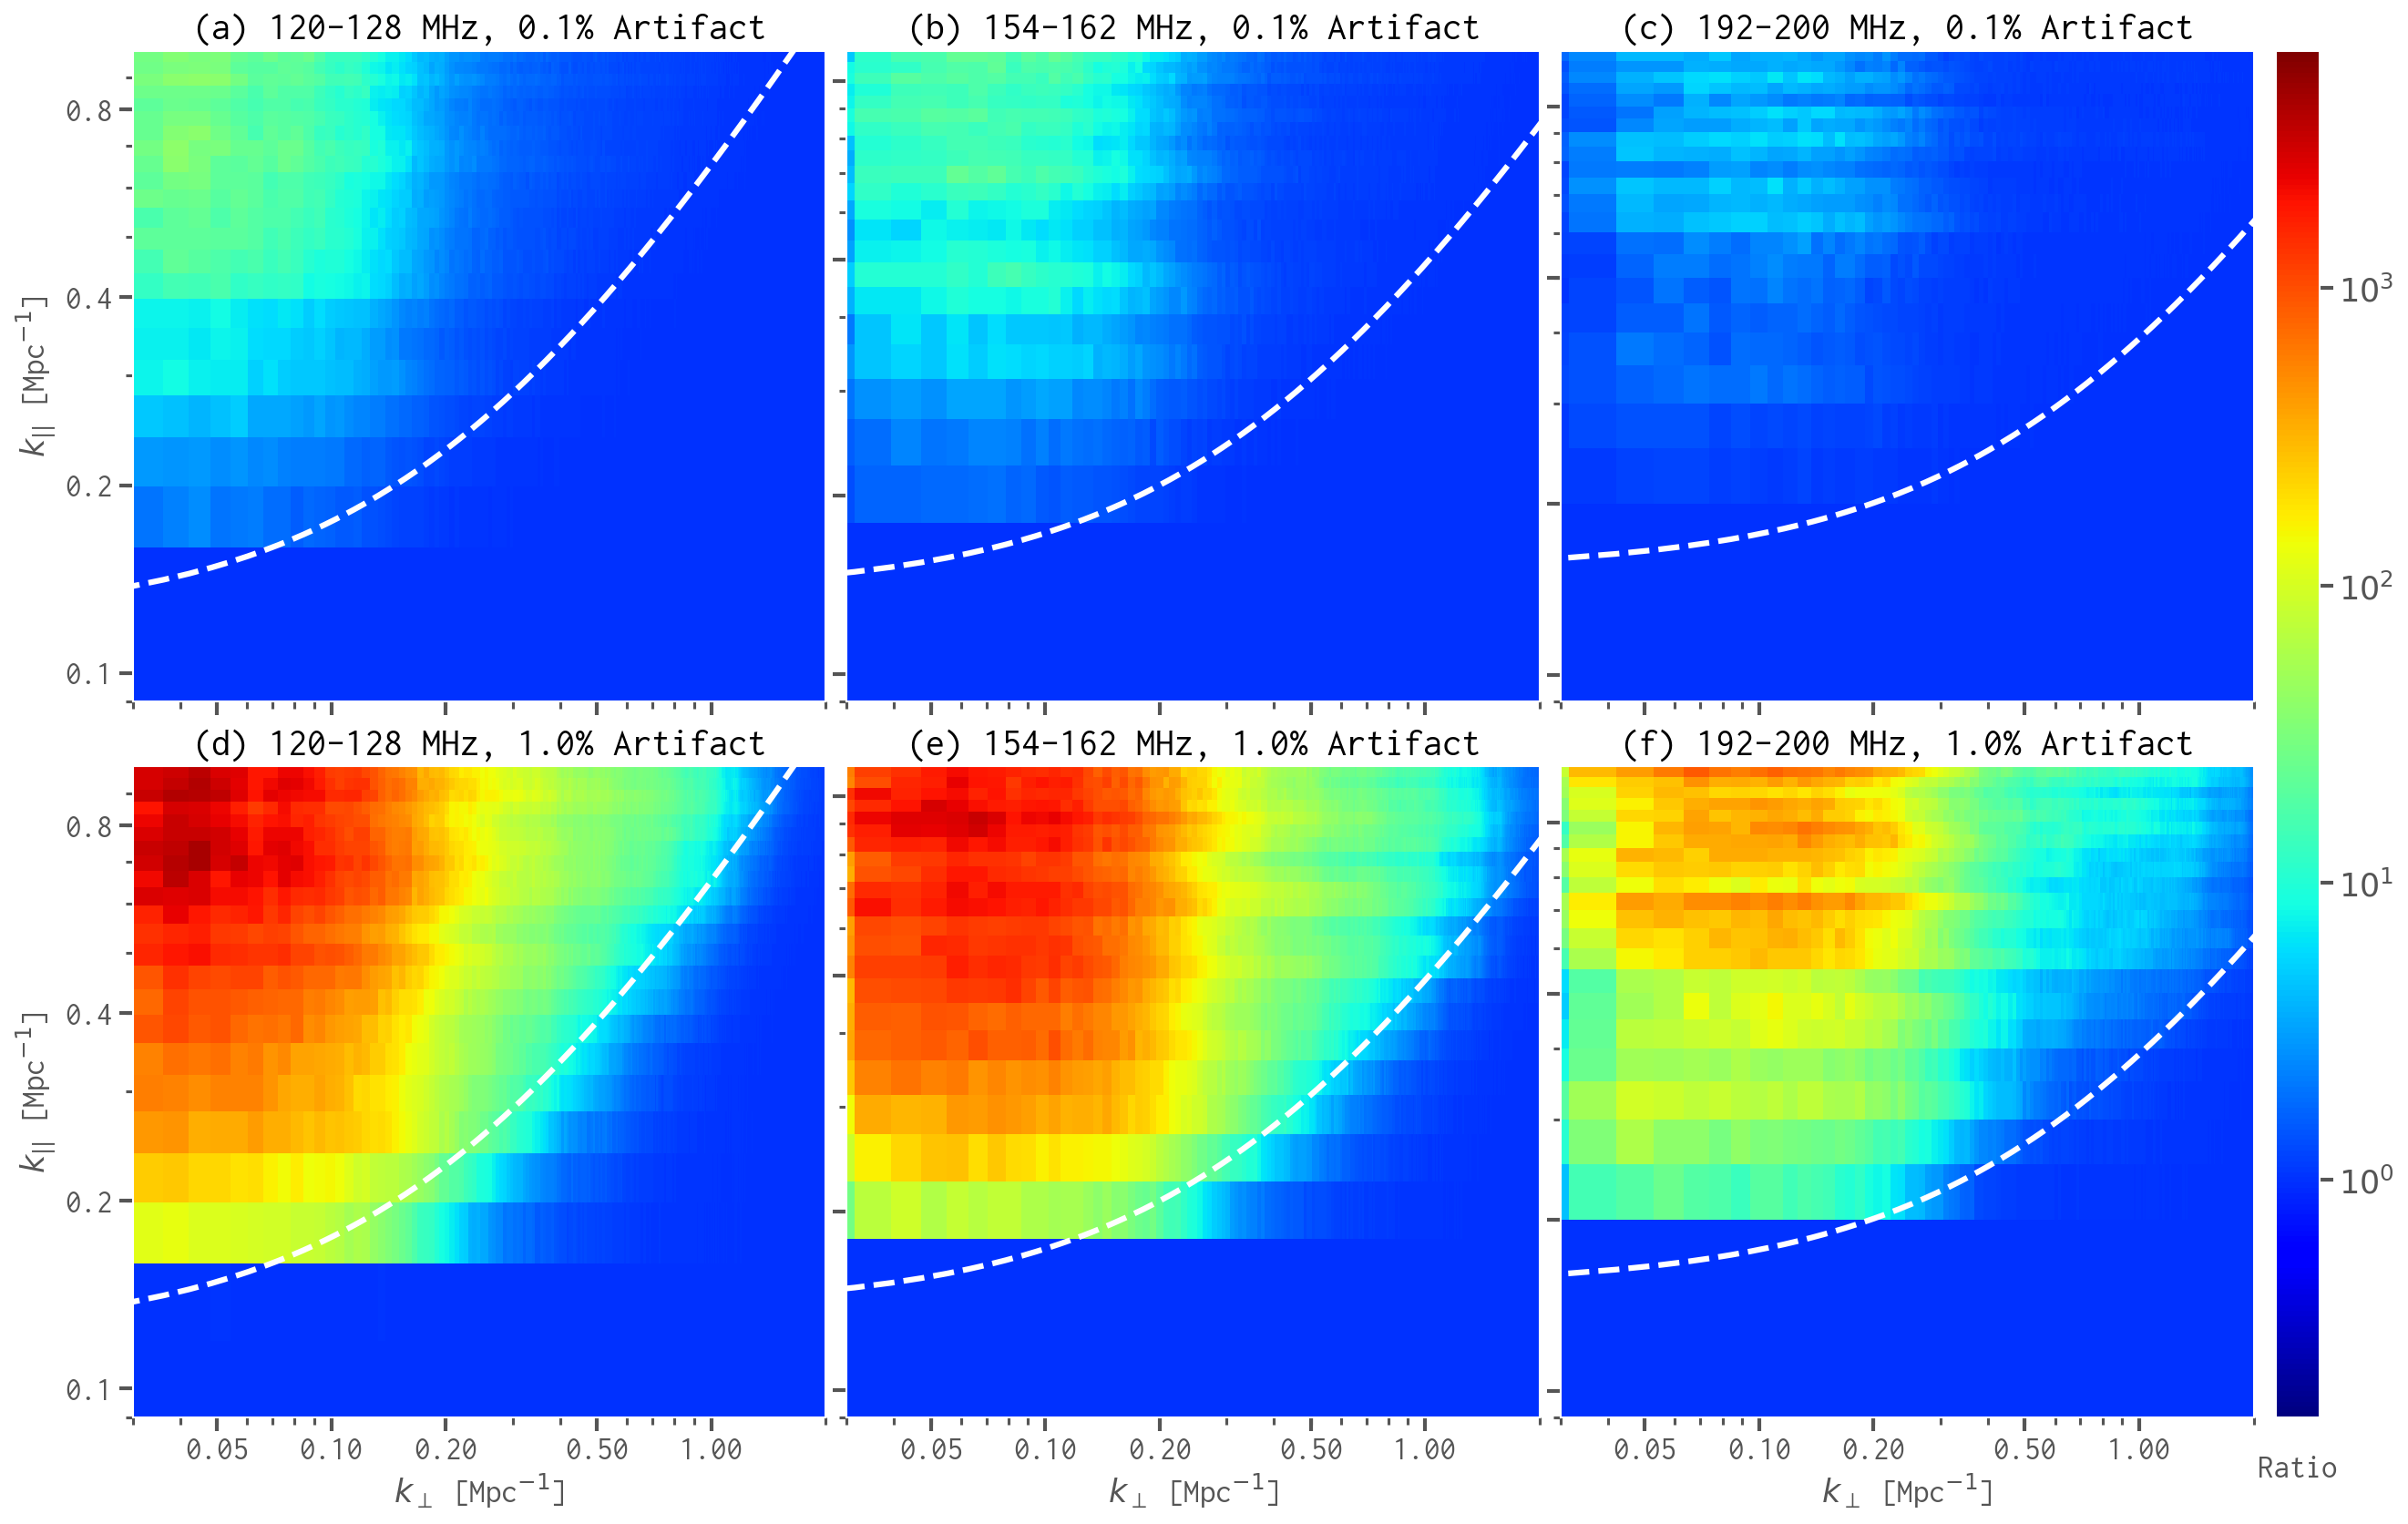
\includegraphics[width=\textwidth]{ps2d-ratio-crp-halos-3bands}
  \caption{\label{fig:ps2d-ratio-crp}%
    2D power spectrum ratios $R_{\R{arti}}(\kperp, \klos)$ of radio
    halos that are obtained between the modified image cubes with
    frequency artifacts and the original ones.
    All the 100 simulation runs for radio halos are used to derive
    the median 2D power spectrum ratios that are presented here.
    The top and bottom rows show the cases of frequency artifacts
    of $A_{\R{arti}} = \SI{0.1}{\percent}$ and
    $A_{\R{arti}} = \SI{1}{\percent}$, respectively.
    The left, middle, and right columns show the power spectrum ratios
    in the \numrange{120}{128}, \numrange{154}{162}, and
    \numrange{192}{200} \si{\MHz} bands.
    The white dashed lines mark the EoR window boundaries.
    All panels share the same color bar in logarithmic scale.
  }
\end{figure*}

To evaluate the influence of the frequency artifacts on the power
spectra, we make use of the image cubes obtained in
\autoref{sec:obs-simu} by multiplying each slice by a random number
drawn from a Gaussian distribution with unity mean and then compare
the resulting power spectra \citep{chapman2016}.
Some simulation and observation studies have suggested that the residual
calibration errors in frequency channels may be about
\SIrange[range-units=repeat]{0.1}{1}{\percent}
\citep[e.g.,][]{barry2016,beardsley2016,ewallWice2017}.
We thus investigate two extreme cases here:
a frequency artifact of amplitude $A_{\R{arti}} = \SI{0.1}{\percent}$ by
using $\sigma = 0.001$ for the Gaussian distribution,
and a frequency artifact of $A_{\R{arti}} = \SI{1}{\percent}$ with
$\sigma = 0.01$.

For each of the 100 simulation runs for radio halos, we calculate the
2D power spectrum ratios $R_{\R{arti}}(\kperp, \klos)$ of the modified
image cube with the frequency artifact to the original one
(\autoref{sec:obs-simu}),
and present the median 2D power spectrum ratios obtained in the
\numrange{120}{128}, \numrange{154}{162}, and \numrange{192}{200}
\si{\MHz} bands with either $A_{\R{arti}} = \SI{0.1}{\percent}$ or
\SI{1}{\percent} in \autoref{fig:ps2d-ratio-crp}.
We find that, when the frequency artifact is added, the resulting 2D
power spectra are seriously damaged in all three frequency bands.
On scales of $\kperp \lesssim \SI{0.2}{\per\Mpc}$ and
$\klos \gtrsim \SI{0.2}{\per\Mpc}$,
when $A_{\R{arti}} = \SI{0.1}{\percent}$ the power of radio halos
becomes about 20, 10, and 3 times stronger in the \numrange{120}{128},
\numrange{154}{162}, and \numrange{192}{200} \si{\MHz} bands,
respectively, and $A_{\R{arti}} = \SI{1}{\percent}$ the corresponding
power increases are about 2000, 1000, and 200 times.
As a comparison, we add the same frequency artifacts
($A_{\R{arti}} = \SI{0.1}{\percent}$ and \SI{1}{\percent}) to the image
cubes of the EoR signal, but find that the changes of the calculated
2D power spectra are very small.
This is because that the EoR signal already fluctuates remarkably along
the frequency dimension.
Therefore, even very minor (\SI{\sim 0.1}{\percent}) instrumental or
calibration uncertainties can make the contamination of radio halos
become much stronger, especially inside the EoR window, where most of the
foreground contamination from our Galaxy and extragalactic point sources
is effectively avoided.
{\color{cyan}%
These results further support our conclusion made in \autoref{sec:ps2d}
that radio halos are important foreground sources and must be carefully
dealt with in the sake of detecting the EoR signal.}

%========================================================================
\subsection{Impacts of Far Side-lobes}
\label{sec:far-sidelobes}
%========================================================================

Phased arrays, which are widely used in low-frequency radio
interferometers (e.g., LOFAR, MWA, SKA1-Low), usually have complicated
beam profiles.
Sources far from the main lobe of the station beam can introduce
noise-like corruptions, known as the far side-lobe confusion noise
(FSCN; \citealt{smirnov2012}), to images through the multitude of
side-lobes.
FSCN will not decrease once the $uv$ coverage of the observation no
longer improves, and can be the limiting factor in the noise
performance of interferometers \citep{mort2017}.

\begin{figure*}
  \centering
  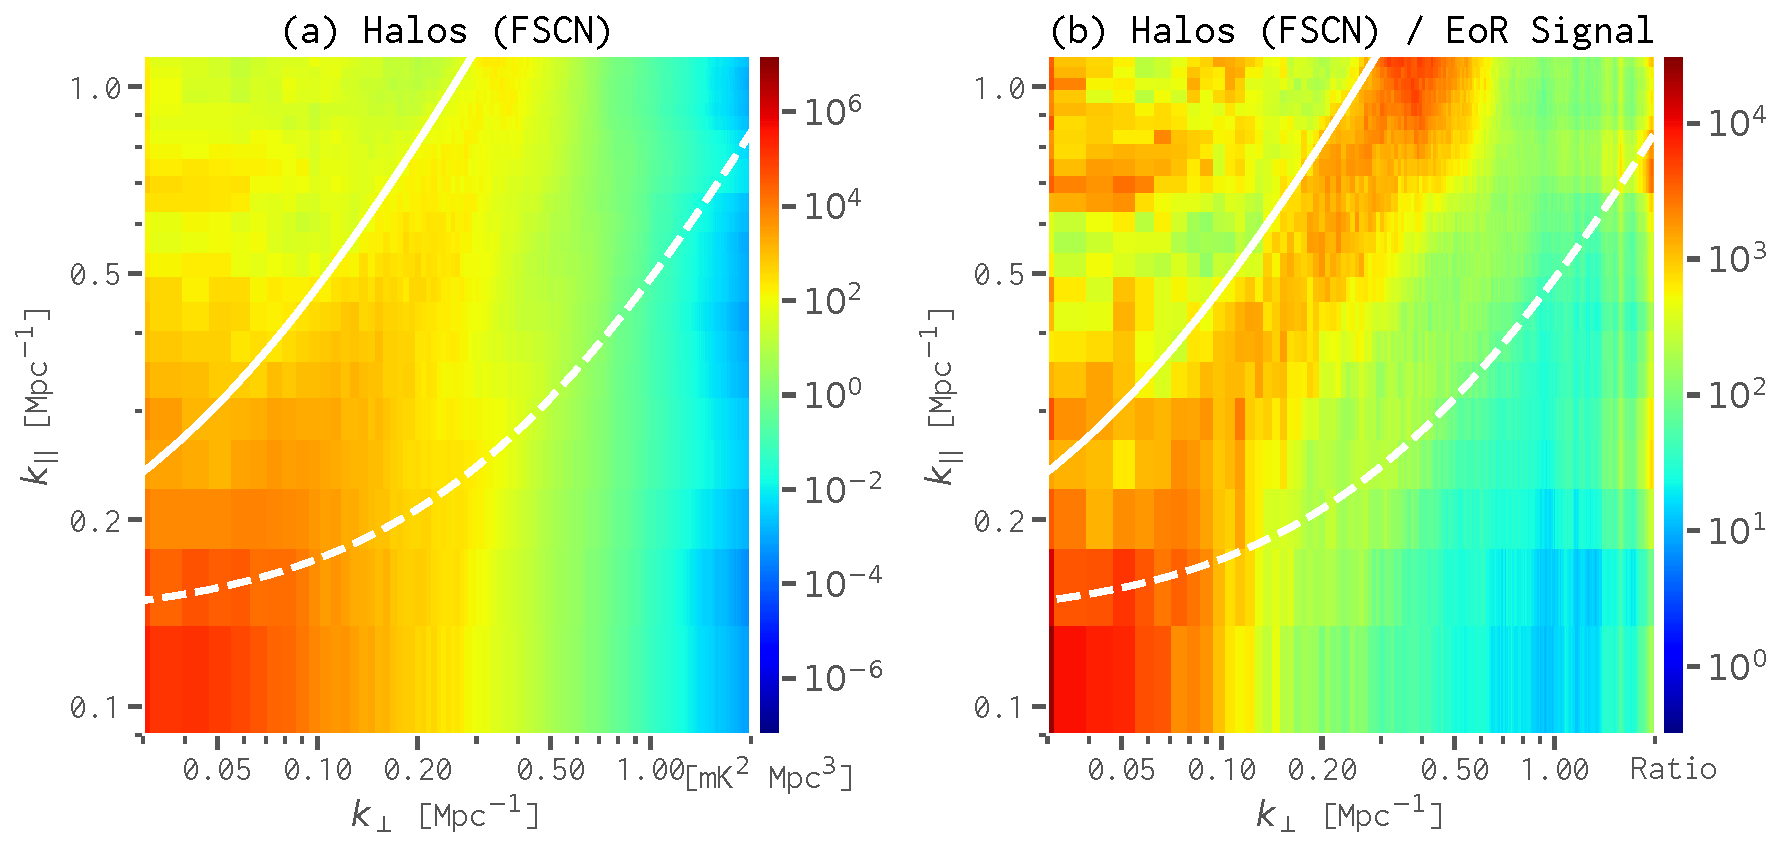
\includegraphics[width=\textwidth]{ps2d-fscn-band158}
  \caption{\label{fig:ps2d-fscn}%
    \textbf{(a)} 2D power spectrum of the FSCN caused by radio halos
    in the far side-lobes of the station beam.
    \textbf{(b)} 2D power spectrum ratio of the FSCN to the EoR signal.
    The results are derived in the \SIrange{154}{162}{\MHz} band.
    The white dashed and solid lines mark the EoR window boundaries
    defined with $\Theta = \SI{6}{\degree}$ and \SI{90}{\degree},
    respectively.
  }
\end{figure*}

To investigate the impacts of FSCN contributed by the radio halos
located in the far side-lobes of the station beam, we have generated
the corresponding sky model for the \texttt{OSKAR} simulator,
which evaluates the radio interferometer measurement equation
\citep{smirnov2011} and is able to perform full-sky simulations with
realistic beam profiles.
More details about the beam shapes and side-lobe properties of the
SKA1-Low can be found in \citet{mort2017}.
As an example, we simulate the radio halos in the \SIrange{154}{162}{\MHz}
band that cover the sky from the edge of the second side-lobe
($\phi \sim \SI{10}{\degree}$ from the field center) to the horizon
($\phi = \SI{90}{\degree}$).
This emulates an ideal CLEAN procedure in practical data analysis that
removes all the radio halos in both the main lobe and the first side-lobe
but leaves the ones in the far side-lobes.
Using the \texttt{OSKAR} simulator and the \texttt{WSClean} imager as
described in \autoref{sec:obs-simu}, we obtain the dirty images of the
central \SI[product-units=repeat]{5 x 5}{\degree} region and then
calculate the 2D power spectrum.

From the 2D power spectrum shown in \autoref{fig:ps2d-fscn}(a),
we find that the FSCN contributed by radio halos is remarkably strong,
and the wedge-shaped contamination region moves toward the top left in
the $(\kperp, \klos)$ plane, which greatly reduces the EoR window.
In order to effectively avoid the FSCN contamination, we are forced to
employ a very conservative EoR window boundary, such as the one defined
with $\Theta = \SI{90}{\degree}$ as marked in \autoref{fig:ps2d-fscn}
with white solid line, at the cost of losing more information of the EoR
signal.
In \autoref{fig:ps2d-fscn}(b), we present the 2D power spectrum ratio
of the FSCN to the EoR signal to better illustrate the impact of the
FSCN on the EoR detection.
It shows that even inside the newly defined EoR window
($\Theta = \SI{90}{\degree}$), the FSCN resulted from radio halos can
be about 1000 times stronger than the EoR signal on scales of
$\kperp \lesssim \SI{0.1}{\per\Mpc}$ and $\klos \gtrsim \SI{0.6}{\per\Mpc}$.
Consequently,
the severe FSCN contamination makes the selection of EoR sky region
a more challenging task, since in principle neither bright radio halos
nor other strong sources are allowed in both the main and side lobes.
A highly accurate foreground model is thus crucial to mitigate the
impacts of FSCN.


%########################################################################
\section{Summary}
\label{sec:summary}
%########################################################################

{\color{cyan}%
In this work, we have simulated the \enquote{observed} image cubes for
the EoR signal, radio halos, Galactic diffuse emission, and extragalactic
point sources by utilizing the latest SKA1-Low layout configuration.
Detailed comparisons of power spectra between radio halos and the EoR
signal as well as other foreground components have been carried out.
We conclude that radio halos are severe foreground sources
to the EoR observations when either foreground removal or foreground
avoidance methods are applied to measure the EoR signal.

The forthcoming low-frequency radio interferometers such as the SKA1-Low
have excellent sensitivity and angular resolution and will provide us
with a unique opportunity to fully explore radio halos in the
low-frequency regime.
The large-scale deep surveys will reveal thousands of radio halos and
enable us to study the underlying physics of radio halos and to build
more accurate foreground model for the EoR observations.
} % cyan


%%%%%%%%%%%%%%%%%%%%%%%%%%%%%%%%%%%%%%%%%%%%%%%%%%%%%%%%%%%%%%%%%%%%%%%%%
\acknowledgments

We would like to thank
Fred Dulwich for providing with the latest SKA1-Low layout configuration
as well as the guidance on using the \texttt{OSKAR} simulator,
Andr\'e Offringa for the help on interferometric imaging with
\texttt{WSClean},
Mathieu Remazeilles for providing us with the high-resolution Haslam
\SI{408}{\MHz} Galactic synchrotron map,
and Giovanna Giardino for the all-sky Galactic synchrotron spectral
index map.
We also acknowledge Emma Chapman, Uri Keshet, and Abhirup Datta for
their help.
Part of the work involving \texttt{OSKAR} and \texttt{WSClean} was
performed on the high-performance cluster at Shanghai Astronomical
Observatory, Chinese Academy of Sciences.
This work is supported by the National Natural Science Foundation of China
(grant Nos. 11433002, 11621303, 61371147),
and the National Key Research and Discovery Plan (grant No. 2017YFF0210903).


%% To help institutions obtain information on the effectiveness of their
%% telescopes the AAS Journals has created a group of keywords for telescope
%% facilities: http://journals.aas.org/authors/aastex/facility.html
%
%% Use \facility{} or \facilities{} macros to list the keywords of facilities
%% used in the research for the paper.  Each keyword is check against the
%% master list during copy editing.  Individual instruments can be provided
%% in parentheses, after the keyword, but they are not verified.

\vspace{5mm}

%% The optional \software command to allow authors a place to specify which
%% programs were used during the creation of the manuscript.  Authors should
%% list each code and include either a citation or url to the code inside ()s
%% when available.

\software{
  OSKAR \citep{mort2010},
  WSClean \citep{offringa2014},
  AstroPy \citep{astropy2013},
  HEALPix \citep{gorski2005},
  HMF \citep{murray2013},
  IPython (\url{https://ipython.org/}),
  Matplotlib (\url{https://matplotlib.org/}),
  NumPy (\url{http://www.numpy.org/}),
  SciPy (\url{https://scipy.org/}),
  Pandas (\url{https://pandas.pydata.org/}).
}


%%%%%%%%%%%%%%%%%%%%%%%%%%%%%%%%%%%%%%%%%%%%%%%%%%%%%%%%%%%%%%%%%%%%%%%%%
%%
%% Appendix material should be preceded with a single \appendix command.
%% There should be a \section command for each appendix. Mark appendix
%% subsections with the same markup you use in the main body of the paper.
%%
%% Each Appendix (indicated with \section) will be lettered A, B, C, etc.
%% The equation counter will reset when it encounters the \appendix
%% command and will number appendix equations (A1), (A2), etc. The
%% Figure and Table counter will not reset.
%%
\appendix

%########################################################################
\section{Collection of Current Observed Radio Halos}
\label{sec:halos-collection}
%########################################################################

\begin{longrotatetable}
\begin{deluxetable*}{lcccr@{$\,\pm\,$}lr@{$\,\pm\,$}lll}
\tabletypesize{\scriptsize}
\tablecaption{\label{tab:halos-observed}%
  Currently Observed 71 Radio Halos and 9 Candidates (As of 2018 January)%
}
\tablehead{
  \colhead{Cluster} &
  \colhead{Redshift} &
  \colhead{kpc/\si{\arcsecond}} &
  \colhead{Size} &
  \multicolumn{2}{c}{$S_{\SI{1.4}{\GHz}}$} &
  \multicolumn{2}{c}{$P_{\SI{1.4}{\GHz}}$} &
  \colhead{Notes} &
  \colhead{References} \\
  \colhead{} &  % cluster
  \colhead{} &  % redshift
  \colhead{} &  % kpc/arcsec
  \colhead{(\si{\Mpc})} &  % size
  \multicolumn{2}{c}{(\si{\mJy})} &  % flux
  \multicolumn{2}{c}{(\SI{e24}{\watt\per\hertz})} &  % power
  \colhead{} &  % notes
  \colhead{} \\
  \colhead{(1)} &
  \colhead{(2)} &
  \colhead{(3)} &
  \colhead{(4)} &
  \multicolumn{2}{c}{(5)} &
  \multicolumn{2}{c}{(6)} &
  \colhead{(7)} &
  \colhead{(8)}
}

\startdata
% Name                 z        kpc/"  size    S1.4   Serr   P1.4     Perr   Notes  Ref
1E 0657$-$56         & 0.2960 & 4.38 & 1.48 &  78.0 &  5.0 & 21.33 &  1.49 &  & \citet{liang2000}  \\
Abell 141            & 0.2300 & 3.64 & 1.20 &   1.3 &  0.1\tablenotemark{a} &  0.25 &  0.02 &  & \citet{duchesne2017}  \\
Abell 209            & 0.2060 & 3.34 & 1.40 &  16.9 &  1.0 &  2.04 &  0.12 & With a relic candidate & \citet{giovannini2009}  \\
Abell 399            & 0.0718 & 1.35 & 0.57 &  16.0 &  2.0 &  0.20 &  0.03 & Double with Abell 401 & \citet{murgia2010}  \\
Abell 401            & 0.0737 & 1.38 & 0.49 &  17.0 &  1.0 &  0.20 &  0.01 & Double with Abell 399 & \citet{bacchi2003}  \\
Abell 520            & 0.1990 & 3.25 & 0.99 &  34.4 &  1.5 &  3.17 &  0.14 &  & \citet{govoni2001}  \\
Abell 521            & 0.2533 & 3.91 & 1.17 &   5.9 &  0.5 &  1.12 &  0.09 & With a relic & \citet{giovannini2009}  \\
Abell 523            & 0.1000 & 1.82 & 1.30 &  59.0 &  5.0 &  1.47 &  0.12 &  & \citet{giovannini2011}  \\
Abell 545            & 0.1540 & 2.64 & 0.81 &  23.0 &  1.0 &  1.25 &  0.05 &  & \citet{bacchi2003}  \\
Abell 665            & 0.1818 & 3.03 & 1.66 &  43.1 &  2.2 &  3.28 &  0.17 &  & \citet{giovannini2000}  \\
Abell 697            & 0.2820 & 4.23 & 0.75 &   5.2 &  0.5 &  2.20 &  0.21 &  & \citet{vanWeeren2011}  \\
Abell 746            & 0.2320 & 3.67 & 0.85 &  18.0 &  4.0 &  3.80 &  0.84 & With a relic & \citet{vanWeeren2011}  \\
Abell 754            & 0.0542 & 1.04 & 0.95 &  86.0 &  4.0 &  0.56 &  0.03 & With a relic & \citet{bacchi2003}  \\
Abell 773            & 0.2170 & 3.48 & 1.13 &  12.7 &  1.3 &  1.39 &  0.14 &  & \citet{govoni2001}  \\
Abell 781            & 0.3004 & 4.42 & 1.60 &  20.5 &  5.0 &  5.90 &  1.44 & With a relic candidate & \citet{govoni2011}  \\
Abell 800            & 0.2223 & 3.55 & 1.28 &  10.6 &  0.9 &  1.52 &  0.13 &  & \citet{govoni2012}  \\
Abell 851            & 0.4069 & 5.40 & 1.08 &   3.7 &  0.3 &  2.14 &  0.17 &  & \citet{giovannini2009}  \\
Abell 1132           & 0.1369 & 2.39 & 0.74 &   3.3 &  1.5 &  0.16 &  0.07 &  & \citet{wilber2018}  \\
Abell 1213           & 0.0469 & 0.91 & 0.22 &  72.2 &  3.5 &  0.36 &  0.02 &  & \citet{giovannini2009}  \\
Abell 1300           & 0.3100 & 4.52 & 0.92 &  20.0 &  2.0 &  2.99 &  0.30 & With a relic & \citet{reid1999}  \\
Abell 1351           & 0.3220 & 4.64 & 1.08 &  32.4 &  --- & 11.37 &  ---  &  & \citet{giacintucci2011b}  \\
Abell 1443           & 0.2700 & 4.10 & 1.10 &  11.0 &  1.1\tablenotemark{b} &  2.53 &  0.30 & Halo candidate & \citet{bonafede2015}  \\
Abell 1451           & 0.1989 & 3.25 & 0.74 &   5.4 &  0.5 &  0.62 &  0.07 & With a relic candidate & \citet{cuciti2018}  \\
Abell 1550           & 0.2540 & 3.92 & 1.41 &   7.7 &  1.6 &  1.49 &  0.31 &  & \citet{govoni2012}  \\
Abell 1656           & 0.0232 & 0.46 & 0.58 & 530.0 & 50.0 &  0.31 &  0.03 & With a relic candidate & \citet{kim1990}  \\
Abell 1682           & 0.2272 & 3.61 & 0.85 &   2.3 &  0.5\tablenotemark{c} &  0.41 &  0.08 & Halo candidate & \citet{macario2013}  \\
Abell 1689           & 0.1832 & 3.05 & 0.73 &  10.0 &  2.9 &  0.92 &  0.27 &  & \citet{vacca2011}  \\
Abell 1758A          & 0.2790 & 4.20 & 0.63 &   3.9 &  0.4 &  0.93 &  0.10 & With a relic & \citet{giovannini2009}  \\
Abell 1914           & 0.1712 & 2.88 & 1.16 &  64.0 &  3.0 &  4.32 &  0.20 &  & \citet{bacchi2003}  \\
Abell 1995           & 0.3186 & 4.61 & 0.83 &   4.1 &  0.7 &  1.35 &  0.23 &  & \citet{giovannini2009}  \\
Abell 2034           & 0.1130 & 2.03 & 0.60 &   7.3 &  2.0 &  0.28 &  0.08 & With a relic & \citet{vanWeeren2011}  \\
Abell 2061           & 0.0784 & 1.46 & 1.68 &  16.9 &  4.2 &  0.25 &  0.06 & With a relic & \citet{farnsworth2013}  \\
Abell 2065           & 0.0726 & 1.36 & 1.08 &  32.9 & 11.0 &  0.41 &  0.14 &  & \citet{farnsworth2013}  \\
Abell 2069           & 0.1160 & 2.08 & 0.90 &   6.2 &  2.2\tablenotemark{d} &  0.25 &  0.05 & Halo may have two components & \citet{drabent2015}  \\
Abell 2142           & 0.0909 & 1.67 & 0.99 &  11.8 &  0.8 &  1.12 &  0.08 & Halo has two components & \citet{venturi2017}  \\
Abell 2163           & 0.2030 & 3.31 & 2.04 & 155.0 &  2.0 & 14.93 &  0.20 & With a relic & \citet{feretti2001}  \\
Abell 2218           & 0.1710 & 2.88 & 0.35 &   4.7 &  0.1 &  0.32 &  0.01 &  & \citet{giovannini2000}  \\
Abell 2219           & 0.2256 & 3.59 & 1.54 &  81.0 &  4.0 &  9.72 &  0.48 &  & \citet{bacchi2003}  \\
Abell 2254           & 0.1780 & 2.98 & 0.85 &  33.7 &  1.8 &  2.43 &  0.13 &  & \citet{govoni2001}  \\
Abell 2255           & 0.0806 & 1.50 & 0.90 &  56.0 &  3.0 &  0.87 &  0.05 & With a relic & \citet{govoni2005}  \\
Abell 2256           & 0.0594 & 1.13 & 0.81 & 103.4 &  1.1 &  0.82 &  0.01 & With a relic & \citet{clarke2006}  \\
Abell 2294           & 0.1780 & 2.98 & 0.54 &   5.8 &  0.5 &  0.51 &  0.04 &  & \citet{giovannini2009}  \\
Abell 2319           & 0.0524 & 1.01 & 0.93 & 153.0 &  8.0 &  0.54 &  0.03 &  & \citet{feretti1997}  \\
Abell 2680           & 0.1901 & 3.14 & 0.57 &   1.8 &  0.6\tablenotemark{e} &  0.16 &  0.05 & Halo candidate & \citet{duchesne2017}  \\
Abell 2693           & 0.1730 & 2.91 & 0.65 &   7.7 &  0.9\tablenotemark{f} &  0.61 &  0.07 & Halo candidate & \citet{duchesne2017}  \\
Abell 2744           & 0.3080 & 4.50 & 1.62 &  57.1 &  2.9 & 12.89 &  0.65 & With a relic & \citet{govoni2001}  \\
Abell 2811           & 0.1080 & 1.95 & 0.48 &   3.4 &  0.7\tablenotemark{g} &  0.10 &  0.02 &  & \citet{duchesne2017}  \\
Abell 3411           & 0.1687 & 2.85 & 0.90 &   4.8 &  0.5 &  0.46 &  0.05 & With a relic & \citet{vanWeeren2013}  \\
Abell 3562           & 0.0480 & 0.93 & 0.44 &  20.0 &  2.0 &  0.10 &  0.01 &  & \citet{venturi2003}  \\
Abell 3888           & 0.1510 & 2.60 & 0.99 &  27.6 &  3.1 &  1.85 &  0.19 &  & \citet{shakouri2016}  \\
Abell S84            & 0.1080 & 1.95 & 0.49 &   2.1 &  0.3\tablenotemark{h} &  0.06 &  0.01 & Halo candidate & \citet{duchesne2017}  \\
Abell S1121          & 0.3580 & 4.98 & 1.25 &   9.8 &  3.1\tablenotemark{h} &  4.54 &  1.44 &  & \citet{duchesne2017}  \\
ACT-CL J0102$-$4915  & 0.8700 & 7.73 & 2.17 &  10.7 &  1.1\tablenotemark{i} & 44.43 &  1.28 & With double relics & \citet{lindner2014}  \\
ACT-CL J0256.5+0006  & 0.3430 & 4.84 & 0.79 &   2.1 &  0.5\tablenotemark{i} &  0.97 &  0.29 &  & \citet{knowles2016}  \\
CIZA J0107.7+5408    & 0.1066 & 1.93 & 1.10 &  55.0 &  5.0 &  1.80 &  0.16 &  & \citet{vanWeeren2011}  \\
CIZA J0638.1+4747    & 0.1740 & 2.92 & 0.59 &   3.6 &  0.2 &  0.30 &  0.02 &  & \citet{cuciti2018}  \\
CIZA J1938.3+5409    & 0.2600 & 3.99 & 0.72 &   1.6 &  0.2\tablenotemark{b} &  0.36 &  0.05 &  & \citet{bonafede2015}  \\
CIZA J2242.8+5301    & 0.1921 & 3.16 & 1.77 &  33.5 &  6.2\tablenotemark{j} &  3.40 &  0.97 & With double relics & \citet{govoni2012}  \\
ClG 0016+16          & 0.5456 & 6.37 & 0.77 &   5.5 &  --- &  4.42 &  ---  &  & \citet{giovannini2000}  \\
ClG 0217+70          & 0.0655 & 1.24 & 0.73 &  58.6 &  0.9 &  0.54 &  0.01 & With double relics & \citet{brown2011}  \\
ClG 1446+26          & 0.3700 & 5.09 & 1.22 &   7.7 &  2.6 &  3.57 &  1.21 & With a relic & \citet{govoni2012}  \\
ClG 1821+64          & 0.2990 & 4.41 & 1.10 &  13.0 &  0.8\tablenotemark{k} &  3.70 &  0.10 &  & \citet{bonafede2014b}  \\
MACS J0416.1$-$2403  & 0.3960 & 5.31 & 0.64 &   1.7 &  0.8\tablenotemark{l} &  1.26 &  0.29 &  & \citet{pandeyPommier2015}  \\
MACS J0520.7$-$1328  & 0.3400 & 4.81 & 0.80 &   9.0 &  1.6 &  3.38 &  0.60 & Halo candidate & \citet{macario2014}  \\
MACS J0553.4$-$3342  & 0.4070 & 5.40 & 1.32 &   9.2 &  0.7\tablenotemark{b} &  6.73 &  0.61 &  & \citet{bonafede2012}  \\
MACS J0717.5+3745    & 0.5458 & 6.37 & 1.20 & 118.0 &  5.0 & 50.00 & 10.00 & With a relic & \citet{vanWeeren2009}  \\
MACS J0949.8+1708    & 0.3825 & 5.20 & 1.04 &   3.1 &  0.3\tablenotemark{b} &  1.63 &  0.15 &  & \citet{bonafede2015}  \\
MACS J1149.5+2223    & 0.5444 & 6.36 & 1.32 &   1.2 &  0.5 &  1.95 &  0.93 & Halo candidate; with double relics & \citet{bonafede2012}  \\
MACS J1752.0+4440    & 0.3660 & 5.05 & 1.65 &  14.2 &  1.4\tablenotemark{m} &  9.50 &  0.91 & With double relics & \citet{vanWeeren2012}  \\
MACS J2243.3$-$0935  & 0.4470 & 5.71 & 0.91 &   3.1 &  0.6\tablenotemark{n} &  3.11 &  0.58 & With a relic candidate & \citet{cantwell2016}  \\
PLCK G147.3$-$16.6   & 0.6500 & 6.92 & 1.80 &   2.5 &  0.4\tablenotemark{o} &  5.10 &  0.80 &  & \citet{vanWeeren2014}  \\
PLCK G171.9$-$40.7   & 0.2700 & 4.10 & 0.99 &  18.0 &  2.0 &  4.76 &  0.10 &  & \citet{giacintucci2013}  \\
PLCK G285.0$-$23.7   & 0.3900 & 5.26 & 0.73 &   2.9 &  0.4\tablenotemark{p} &  1.67 &  0.21 &  & \citet{martinezAviles2016}  \\
PLCK G287.0+32.9     & 0.3900 & 5.26 & 1.30 &   8.8 &  0.9 &  5.10 &  0.51 & With double relics & \citet{bonafede2014a}  \\
PSZ1 G108.18$-$11.53 & 0.3347 & 4.77 & 0.84 &   6.8 &  0.2 &  2.72 &  0.10 & With double relics & \citet{deGasperin2015}  \\
RXC J1234.2+0947     & 0.2290 & 3.63 & 0.92 &   2.0 &  --- &  0.30 &  ---  & Halo candidate & \citet{govoni2012}  \\
RXC J1314.4$-$2515   & 0.2474 & 3.85 & 1.27 &  20.3 &  0.8 &  1.45 &  0.06 & With double relics & \citet{feretti2005}  \\
RXC J1514.9$-$1523   & 0.2226 & 3.55 & 1.38 &  10.0 &  2.0 &  1.65 &  0.33 &  & \citet{giacintucci2011a}  \\
RXC J2003.5$-$2323   & 0.3171 & 4.59 & 1.38 &  35.0 &  2.0 & 11.96 &  0.68 &  & \citet{giacintucci2009}  \\
RXC J2351.0$-$1954   & 0.2477 & 3.85 & 0.64 &   4.5 &  0.9\tablenotemark{q} &  0.89 &  0.18 & Halo candidate & \citet{duchesne2017}  \\
\enddata

\tablenotetext{a}{Extrapolated from \SI{168}{\MHz} with spectral index $\alpha=2.1$.}
\tablenotetext{b}{Extrapolated from \SI{323}{\MHz} with spectral index $\alpha=1.3$.}
\tablenotetext{c}{Extrapolated from \SI{153}{\MHz} with spectral index $\alpha=1.7$.}
\tablenotetext{d}{Extrapolated from \SI{346}{\MHz} with spectral index $\alpha=1.0$.}
\tablenotetext{e}{Extrapolated from \SI{168}{\MHz} with spectral index $\alpha=1.2$.}
\tablenotetext{f}{Extrapolated from \SI{168}{\MHz} with spectral index $\alpha=0.88$.}
\tablenotetext{g}{Extrapolated from \SI{168}{\MHz} with spectral index $\alpha=1.5$.}
\tablenotetext{h}{Extrapolated from \SI{168}{\MHz} with spectral index $\alpha=1.3$.}
\tablenotetext{i}{Extrapolated from \SI{610}{\MHz} with spectral index $\alpha=1.2$.}
\tablenotetext{j}{Extrapolated from \SI{145}{\MHz} with spectral index $\alpha=1.03$.}
\tablenotetext{k}{Extrapolated from \SI{325}{\MHz} with spectral index $\alpha=1.04$.}
\tablenotetext{l}{Extrapolated from \SI{340}{\MHz} with spectral index $\alpha=1.5$.}
\tablenotetext{m}{Extrapolated from \SI{1714}{\MHz} with spectral index $\alpha=1.1$.}
\tablenotetext{o}{Extrapolated from \SI{610}{\MHz} with spectral index $\alpha=1.4$.}
\tablenotetext{p}{Extrapolated from \SI{1867}{\MHz} with spectral index $\alpha=1.3$.}
\tablenotetext{q}{Extrapolated from \SI{168}{\MHz} with spectral index $\alpha=1.4$.}
\tablecomments{\textbf{Columns:}
  \textbf{(1)} galaxy cluster name;
  \textbf{(2)} redshift;
  \textbf{(3)} \si{\kpc} per \si{\arcsec} at the cluster's redshift
               (converted to our adopted cosmology);
  \textbf{(4)} largest linear size of the observed radio halo, in units of \si{\Mpc};
  \textbf{(5)} measured flux density and the uncertainty at \SI{1.4}{\GHz};
  \textbf{(6)} \SI{1.4}{\GHz} radio power and the uncertainty
               (converted to our adopted cosmology);
  \textbf{(7)} extra notes;
  \textbf{(8)} references to the quoted halo properties.
}
\end{deluxetable*}
\end{longrotatetable}


%########################################################################
\section{Supplemental Formulas}
\label{sec:formulas}
%########################################################################

In a flat \lcdm{} cosmology as adopted in this work, the critical linear
overdensity as a function of redshift $z$ is \citep{kitayama1996,randall2002}
\begin{equation}
  \label{eq:delta-crit}
  \delta_c(z) = \frac{D(z=0)}{D(z)} \frac{3}{20} (12\pi)^{2/3}
    \left[1 + 0.0123 \log_{10} \Omega_f(z) \right],
\end{equation}
where $\Omega_f(z)$ is the mass density ratio at redshift $z$ defined as
\begin{equation}
  \label{eq:omega-fz}
  \Omega_f(z) = \frac{\Omega_m(1+z)^3}{\Omega_m(1+z)^3 + \Omega_{\Lambda}},
\end{equation}
and $D(z)$ is the growth factor given by \citep[equation~(13.6)]{peebles1980}
\begin{equation}
  \label{eq:growth-factor}
  D(x) = \frac{(x^3 + 2)^{1/2}}{x^{3/2}}
    \int_0^x y^{3/2} (y^3 + 2)^{-3/2} \,\D{y},
\end{equation}
with $x_0 \equiv (2\Omega_{\Lambda}/\Omega_m)^{1/3}$ and $x = x_0 / (1+z)$.

The Hubble parameter at redshift $z$ is
\begin{equation}
  \label{eq:hubble-z}
  H(z) = H_0 E(z) = H_0 \sqrt{\Omega_m(1+z)^3 + \Omega_{\Lambda}} \,,
\end{equation}
where $E(z)$ is the redshift evolution factor \citep{hogg1999}.

The virial radius of a galaxy cluster is defined as
\begin{equation}
  \label{eq:radius-virial}
  r_{\R{vir}} = \left[
    \frac{3 M_{\R{vir}}}{4\pi \,\Delta_{\R{vir}}(z) \rho_{\R{crit}}(z)}
  \right]^{1/3},
\end{equation}
where $M_{\R{vir}}$ is the virial mass of the cluster,
$\rho_{\R{crit}}(z) = 3 H^2(z) / (8\pi G)$ is the critical density
at redshift $z$ with $G$ being the gravitational constant,
and $\Delta_{\R{vir}}(z)$ is the average overdensity of the cluster
given by \citep{kitayama1996,cassano2005}
\begin{equation}
  \label{eq:delta-vir}
  \Delta_{\R{vir}}(z) = 18\pi^2 \left[ 1 + 0.4093 \, w(z)^{0.9052} \right],
\end{equation}
where $w(z) \equiv \Omega_f^{-1}(z) - 1$.


%%%%%%%%%%%%%%%%%%%%%%%%%%%%%%%%%%%%%%%%%%%%%%%%%%%%%%%%%%%%%%%%%%%%%%%%%
\bibliography{references}


%% Include this line if you are using the \added, \replaced, \deleted
%% commands to see a summary list of all changes at the end of the article.
%\listofchanges

\end{document}

%% EOF
